%%%%%%%%%%%%%%%%%%%%%%%%%%%%%%%%%%%%%%%%%
% Short Sectioned Assignment LaTeX Template Version 1.0 (5/5/12)
% This template has been downloaded from: http://www.LaTeXTemplates.com
% Original author:  Frits Wenneker (http://www.howtotex.com)
% License: CC BY-NC-SA 3.0 (http://creativecommons.org/licenses/by-nc-sa/3.0/)
%%%%%%%%%%%%%%%%%%%%%%%%%%%%%%%%%%%%%%%%%

%----------------------------------------------------------------------------------------
%	PACKAGES AND OTHER DOCUMENT CONFIGURATIONS
%----------------------------------------------------------------------------------------

\documentclass[paper=a4, fontsize=11pt]{scrartcl} % A4 paper and 11pt font size

% ---- Entrada y salida de texto -----

\usepackage{hyperref}
\usepackage{varioref}
\usepackage[T1]{fontenc} % Use 8-bit encoding that has 256 glyphs
\usepackage[utf8]{inputenc}
%\usepackage{fourier} % Use the Adobe Utopia font for the document - comment this line to return to the LaTeX default

% ---- Idioma --------

\usepackage[spanish, es-tabla]{babel} % Selecciona el español para palabras introducidas automáticamente, p.ej. "septiembre" en la fecha y especifica que se use la palabra Tabla en vez de Cuadro

% ---- Otros paquetes ----

\usepackage{amsmath,amsfonts,amsthm} % Math packages
%\usepackage{graphics,graphicx, floatrow} %para incluir imágenes y notas en las imágenes
\usepackage{graphics,graphicx, float} %para incluir imágenes y colocarlas

% Para hacer tablas comlejas
%\usepackage{multirow}
%\usepackage{threeparttable}

%\usepackage{sectsty} % Allows customizing section commands
%\allsectionsfont{\centering \normalfont\scshape} % Make all sections centered, the default font and small caps

\usepackage{fancyhdr} % Custom headers and footers
\pagestyle{fancyplain} % Makes all pages in the document conform to the custom headers and footers
\fancyhead{} % No page header - if you want one, create it in the same way as the footers below
\fancyfoot[L]{} % Empty left footer
\fancyfoot[C]{} % Empty center footer
\fancyfoot[R]{\thepage} % Page numbering for right footer
\renewcommand{\headrulewidth}{0pt} % Remove header underlines
\renewcommand{\footrulewidth}{0pt} % Remove footer underlines
\setlength{\headheight}{13.6pt} % Customize the height of the header

\numberwithin{equation}{section} % Number equations within sections (i.e. 1.1, 1.2, 2.1, 2.2 instead of 1, 2, 3, 4)
\numberwithin{figure}{section} % Number figures within sections (i.e. 1.1, 1.2, 2.1, 2.2 instead of 1, 2, 3, 4)
\numberwithin{table}{section} % Number tables within sections (i.e. 1.1, 1.2, 2.1, 2.2 instead of 1, 2, 3, 4)

\setlength\parindent{0pt} % Removes all indentation from paragraphs - comment this line for an assignment with lots of text

\newcommand{\horrule}[1]{\rule{\linewidth}{#1}} % Create horizontal rule command with 1 argument of height


%----------------------------------------------------------------------------------------
%	TÍTULO Y DATOS DEL ALUMNO
%----------------------------------------------------------------------------------------

\title{	
\normalfont \normalsize 
\textsc{{\bf Ingeniería de Servidores (2015-2016)} \\ Grado en Ingeniería Informática \\ Universidad de Granada} \\ [25pt] % Your university, school and/or department name(s)
\horrule{0.5pt} \\[0.4cm] % Thin top horizontal rule
\huge Memoria Práctica 3 \\ % The assignment title
\horrule{2pt} \\[0.5cm] % Thick bottom horizontal rule
}

\author{Francisco Carrillo Pérez} % Nombre y apellidos

\date{\normalsize\today} % Incluye la fecha actual

%----------------------------------------------------------------------------------------
% DOCUMENTO
%----------------------------------------------------------------------------------------

\begin{document}

\maketitle % Muestra el Título

\newpage %inserta un salto de página

\tableofcontents % para generar el índice de contenidos

\listoffigures

\listoftables

\newpage

%%%%%%%%%%%%%%%%%%%%%%%%%%%%%%%%%%%%%%%%%%%%%%%%%%%%
% CUESTIÓN 1
%%%%%%%%%%%%%%%%%%%%%%%%%%%%%%%%%%%%%%%%%%%%%%%%%%%%

\section{Cuestión 1:}
\subsection{¿Qué archivo le permite ver qué programas se han instalado con el gestor de paquetes?}
Siguiendo las pistas que se encuentran en el párrafo superior a  esta pregunta, podemos encontrar que el archivo que permite visualizar los programas que se han instalado con el gestor de paquetes es el \textbf{/var/log/apt/history.log} , donde podemos encontrar el comando que se utilizó para instalar el programa, que programa se instaló, a que hora...
\begin{figure}[H] %con el [H] le obligamos a situar aquí la figura
	\centering
	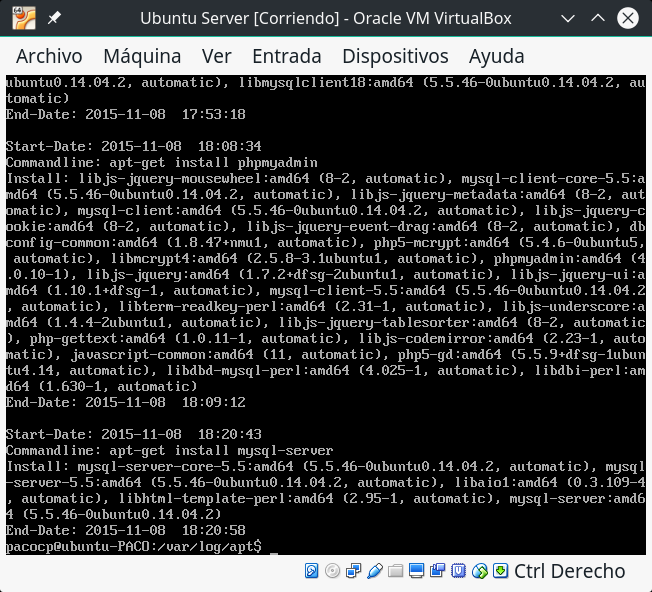
\includegraphics[scale=0.5]{figuras/figura43.png}  %el parámetro scale permite agrandar o achicar la imagen. En el nombre de archivo puede especificar directorios
	\label{figura43}
	
	\caption{Lo que podemos observar usando el comando \textbf{cat /var/log/apt/history.log}} 
\end{figure}

En cambio, en CentOS para poder ver los programas que se han instalado tenemos que ver el archivo \textbf{/var/log/yum.log}, donde podemos ver toda la información.
\begin{figure}[H] %con el [H] le obligamos a situar aquí la figura
	\centering
	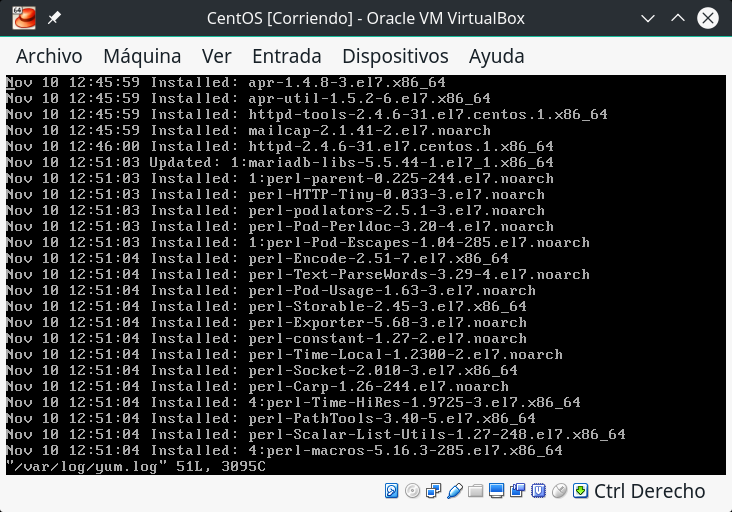
\includegraphics[scale=0.5]{figuras/figura48.png}  %el parámetro scale permite agrandar o achicar la imagen. En el nombre de archivo puede especificar directorios
	\label{figura48}
	
	\caption{Lo que podemos observar usando el comando \textbf{cat /var/log/yum.log}} 
\end{figure}
\subsection{¿Qué significan las terminaciones .1.gz o .2.gz de los archivos en ese directorio?}
Esto se basa en el comando logrotated \cite{logrotated}, estas terminaciones tienen que ver con la antigüedad de los log que se encuentran dentro de estos archivos comprimidos. A diferencia de lo que se podría pensar, los más antigüos son aquellos con un número superior, mientras que los más nuevos son aquellos con el número menor. Por eso el término logrotated, se va produciendo una rotación en los logs renombrando.

%%%%%%%%%%%%%%%%%%%%%%%%%%%%%%%%%%%%%%%%%%%%%%%%%%%%
% CUESTIÓN 2
%%%%%%%%%%%%%%%%%%%%%%%%%%%%%%%%%%%%%%%%%%%%%%%%%%%%
\section{Cuestión 2: ¿qué archivo ha de modificar para programar una tarea? Escriba la línea necesaria para ejecutar una vez al día una copia del directorio ~/codigo a ~/seguridad/$fecha donde $fecha es la fecha actual (puede usar el comando date).}
El archivo que hay que modificar es: \textbf{/tmp/crontab.Ke9pGF/crontab} \cite{crontab}
Sabemos que hay que modificar este archivo ya que  utilizando el comando \textbf{crontab -e} \cite{crontab2} es el archivo que se nos abre.\\
Ahora vamos a crear el script que vamos a ejecutar para realizar la tarea asignada. El mismo sería el de la Figura 2.1.

\begin{figure}[H] %con el [H] le obligamos a situar aquí la figura
	\centering
	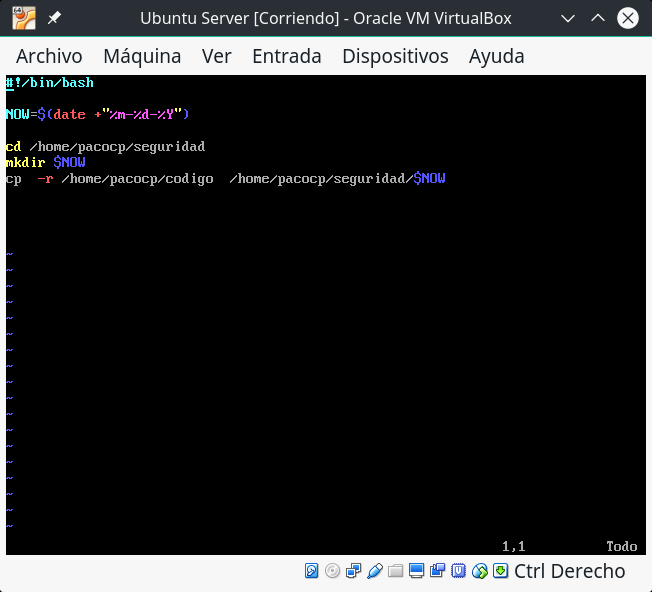
\includegraphics[scale=0.5]{figuras/figura47.png}  %el parámetro scale permite agrandar o achicar la imagen. En el nombre de archivo puede especificar directorios
	\label{figura47}
	
	\caption{Script para realizar la copia de seguridad} 
\end{figure}
Para añadir la línea podemos guiarnos por las líneas que ya vienen por defecto en el contrab de Ubuntu Server:\\
\textbf{55 23 * * * root  /home/pacocp/script.sh}\\

Esto haría que todos los días a las 23:55 se ejecutara el comando.
\begin{figure}[H] %con el [H] le obligamos a situar aquí la figura
	\centering
	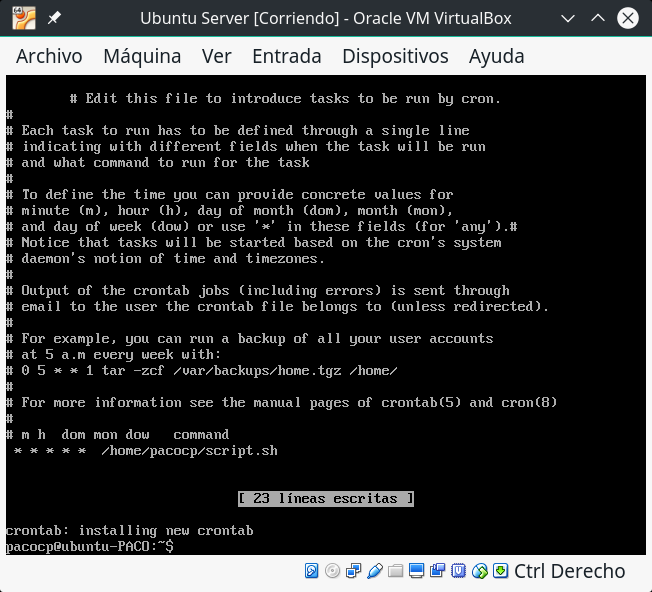
\includegraphics[scale=0.5]{figuras/figura45.png}  %el parámetro scale permite agrandar o achicar la imagen. En el nombre de archivo puede especificar directorios
	\label{figura1}
	
	\caption{Así quedaría el archivo contrab después de ejecutar \textbf{crontab -e}} 
\end{figure}

Entonces, en la Figura 2.3 podemos observar que ocurriría cuando se ejecutara el cron.
\begin{figure}[H] %con el [H] le obligamos a situar aquí la figura
	\centering
	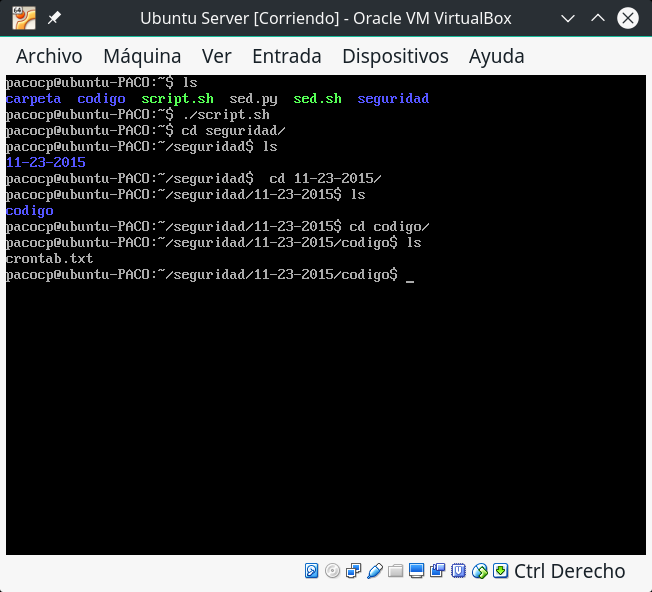
\includegraphics[scale=0.5]{figuras/figura46.png}  %el parámetro scale permite agrandar o achicar la imagen. En el nombre de archivo puede especificar directorios
	\label{figura46}
	
	\caption{Podemos observar lo que realiza el cron} 
\end{figure}
%%%%%%%%%%%%%%%%%%%%%%%%%%%%%%%%%%%%%%%%%%%%%%%%%%%%
% CUESTIÓN 3
%%%%%%%%%%%%%%%%%%%%%%%%%%%%%%%%%%%%%%%%%%%%%%%%%%%%
\section{Cuestión 3: Pruebe a ejecutar el comando, conectar un dispositivo USB y vuelva a ejecutar el comando. Copie y pegue la salida del comando. (considere usar dmesg | tail). Comente qué observa en la información mostrada.}
Primero vamos a ejecutar el comando sin conectar el dispositivo USB:
\textbf{dmesg | tail}\\
\begin{figure}[H] %con el [H] le obligamos a situar aquí la figura
	\centering
	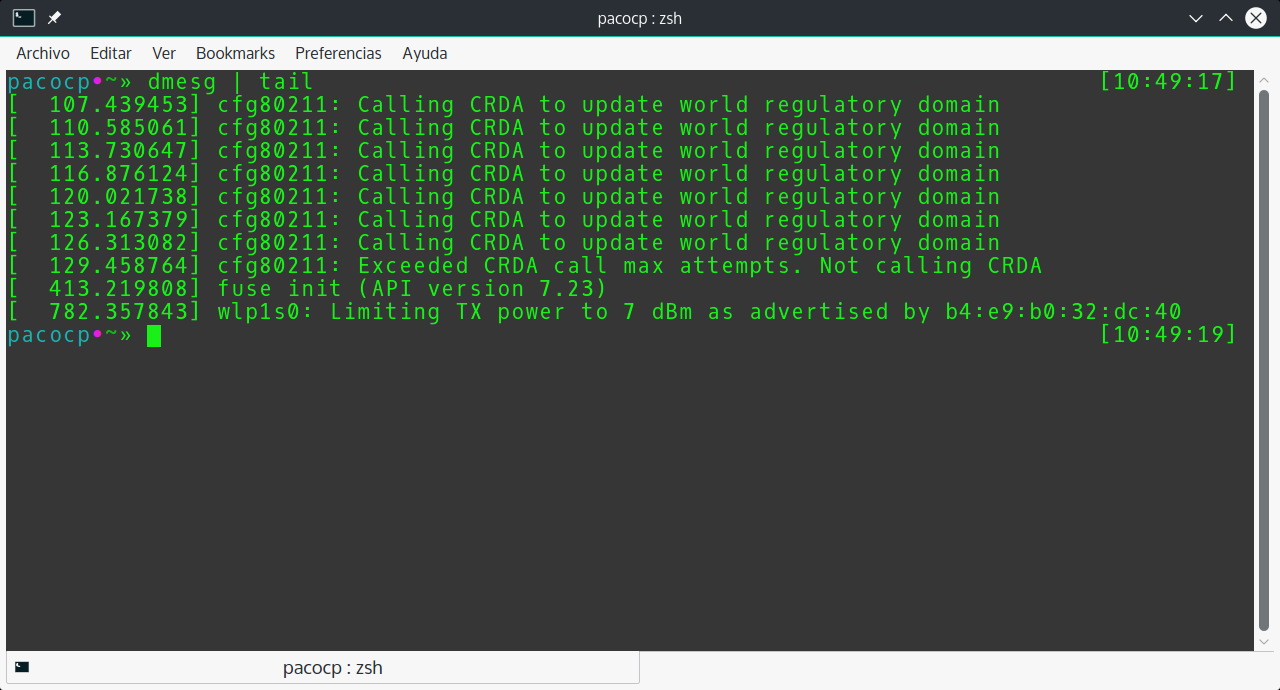
\includegraphics[scale=0.5]{figuras/figura2.png}  %el parámetro scale permite agrandar o achicar la imagen. En el nombre de archivo puede especificar directorios
	\label{figura2}
	
	\caption{Observamos como nos muestra los datos, en este caso de una red que tengo configurada } 
\end{figure}

\begin{figure}[H] %con el [H] le obligamos a situar aquí la figura
	\centering
	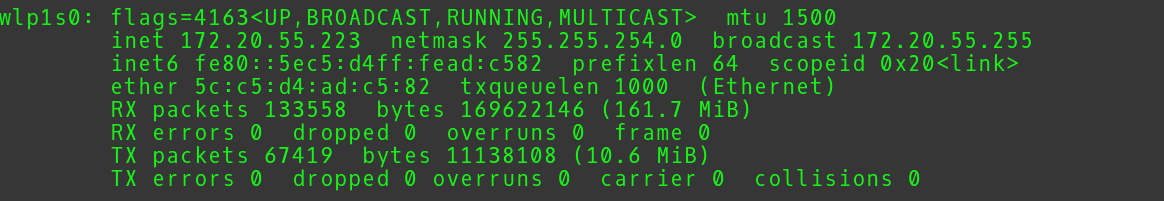
\includegraphics[scale=0.5]{figuras/figura4.png}  %el parámetro scale permite agrandar o achicar la imagen. En el nombre de archivo puede especificar directorios
	\label{figura4}
	
	\caption{Aquí podemos observar la red que tengo configurada llamada wlp1s0} 
\end{figure}

Ahora si conectamos el dispositivo USB vamos a observar como se van a ir realizando todas las operaciones:
\begin{enumerate}
	\item se registra una nueva interfaz de almacenamiento usb.
	\item Te dice el nombre en este caso SanDisl Cruzer Blade.
	\item indica la capacidad del dispositivo, en este caso 32.0 GB.
	\item Te indica que la protección de escritura está desactivada, por lo que se pueden escribir datos en él.
	\item El mode sense que nos devuelve algunos parámetros y características del USB \cite{modesense}.
	\item La escritura en caché está desactivada y la lectura en caché activada.
	\item Donde se encuentra montado el dispositivo, en sdb1 en mi caso.
	\item Que es un disco que se puede retirar.
	\item Por último, un error que nos dice que no fue correctamente desmontado, aunque en ningún caso lo ha sido todavía.
\end{enumerate}
\begin{figure}[H] %con el [H] le obligamos a situar aquí la figura
	\centering
	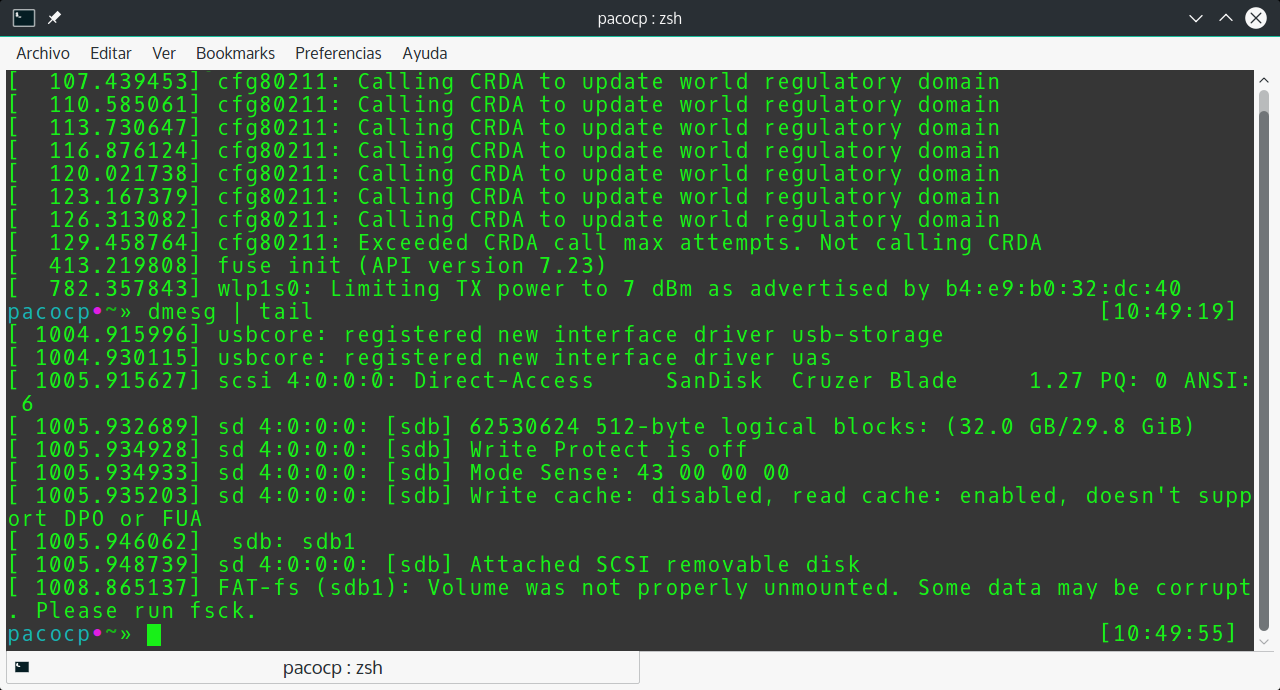
\includegraphics[scale=0.5]{figuras/figura3.png}  %el parámetro scale permite agrandar o achicar la imagen. En el nombre de archivo puede especificar directorios
	\label{figura3}
	
	\caption{Toda la información al hacer dmesg | tail al haber introducido el dispositivo USB} 
\end{figure}

%%%%%%%%%%%%%%%%%%%%%%%%%%%%%%%%%%%%%%%%%%%%%%%%%%%%
% CUESTIÓN 4
%%%%%%%%%%%%%%%%%%%%%%%%%%%%%%%%%%%%%%%%%%%%%%%%%%%%

\section{Cuestión 4: Ejecute el monitor de “System Performance” y muestre el resultado. Incluya capturas de pantalla comentando la información que aparece.}

\begin{figure}[H] %con el [H] le obligamos a situar aquí la figura
	\centering
	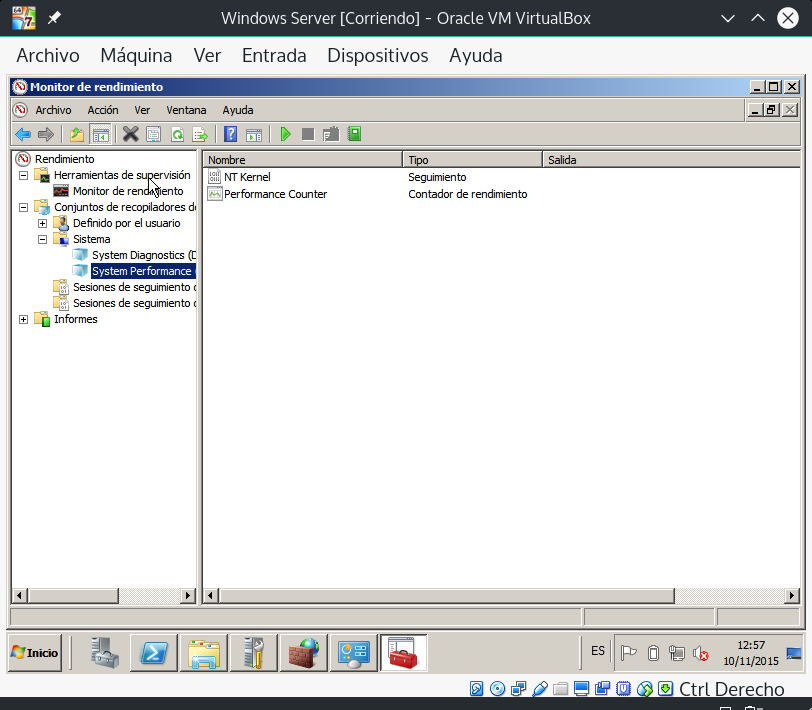
\includegraphics[scale=0.5]{figuras/figura5.png}  %el parámetro scale permite agrandar o achicar la imagen. En el nombre de archivo puede especificar directorios
	\label{figura5}
	
	\caption{Para ejecutar el monitor le damos click con el botón derecho e iniciar.} 
\end{figure}

Una vez que ya lo hemos iniciado, cuando queramos, volviendo a hacer click derecho y pulsamos en detener para que pare la recopilación de información.\\
Si vemos el archivo que se ha generado podemos observar la información recopilada e interpretarla:\\

Podemos observar que lo primero que nos aparece es un Informe de rendimiento del sistema donde nos encontramos información sobre el equipo, el día y hora de la recopilación y la duración de la recopilación.\\
Debajo, nos encontramos con un pequeño resumen de la información más importante,
según que:\\
\begin{itemize}
	\item Proceso: como el Total de \% de CPU que en este caso es 3\%
	\item Disco: con información sobre las entradas salidas en disco, en este caso han sido 61, y la longitud de la cola de disco, al haber sido un dignóstico muy corto solo es 1.
	\item Memoria:con un 79\% de uso, los 512MB de RAM que le dimos a la máquina virtual y el proceso más frecuente, que en este caso ha sido la powershell.
	\item Red: Donde nos dice las direcciones IP de salida y entrada más solicitadas y de donde han recibido más paquetes, que en este caso es la IP \textbf{204.79.197.200} que es la de la página Bing, ya que es la de inicio cuando abrimos el navegador Internet Explorer.
\end{itemize} 
\begin{figure}[H] %con el [H] le obligamos a situar aquí la figura
	\centering
	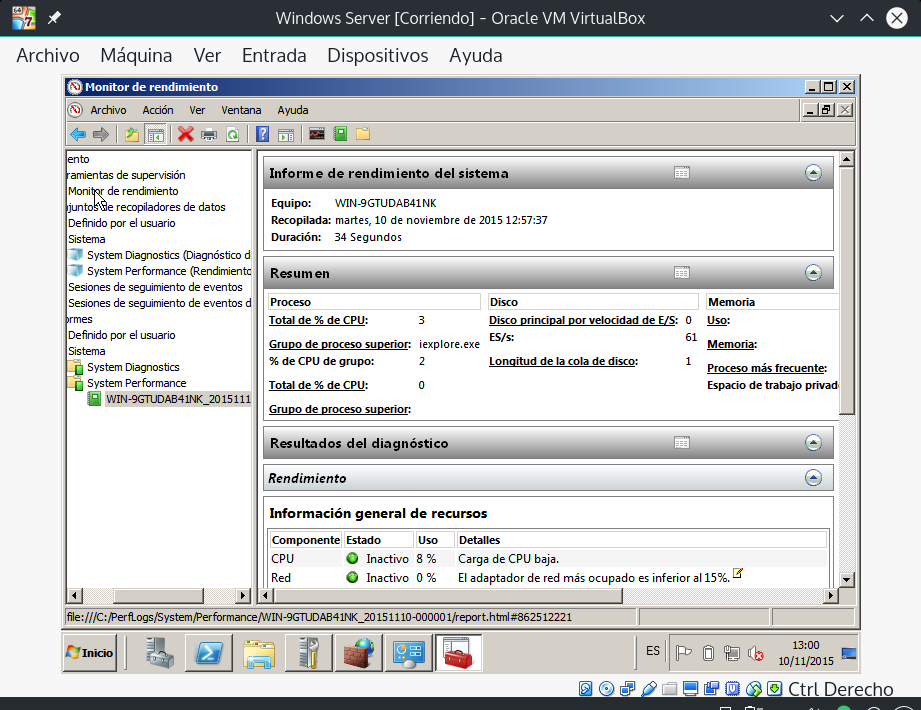
\includegraphics[scale=0.5]{figuras/figura6.png}  %el parámetro scale permite agrandar o achicar la imagen. En el nombre de archivo puede especificar directorios
	\label{figura6}
	
	\caption{Primera parte con informe de rendimiento del sistema y un resumen} 
\end{figure}

\begin{figure}[H] %con el [H] le obligamos a situar aquí la figura
	\centering
	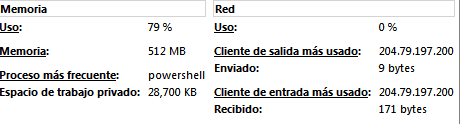
\includegraphics[scale=0.8]{figuras/figura9.png}  %el parámetro scale permite agrandar o achicar la imagen. En el nombre de archivo puede especificar directorios
	\label{figura9}
	
	\caption{Segunda parte con memoria y redes} 
\end{figure}

Más abajo nos encontramos con los Resultados del Diagnóstico. En la Figura 4.4  podemos observar la información general de recursos donde nos dice detalles exactos de lo anteriormente expuesto, como que la carga de CPU era baja, que el adaptador de red más ocupado es inferior al 15\% o que la cantidad de memoria que teníamos disponible era de 107MB.\\
Por último, en la Figura 4.5 podemos observar el id por ejemplo del proceso de Internet Explorer, la cantidad de subprocesos que ha generado, y cuántos de esos ha utilizado. Y también características interesantes como el \% de CPU usado por el Kernel y cuanto por procesos de usuario.
\begin{figure}[H] %con el [H] le obligamos a situar aquí la figura
	\centering
	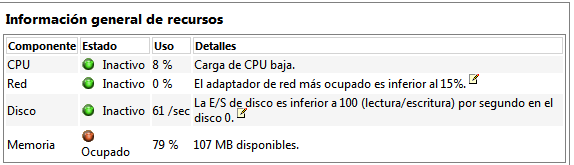
\includegraphics[scale=0.5]{figuras/figura8.png}  %el parámetro scale permite agrandar o achicar la imagen. En el nombre de archivo puede especificar directorios
	\label{figura8}
	
	\caption{Información general de recursos} 
\end{figure}
\begin{figure}[H] %con el [H] le obligamos a situar aquí la figura
	\centering
	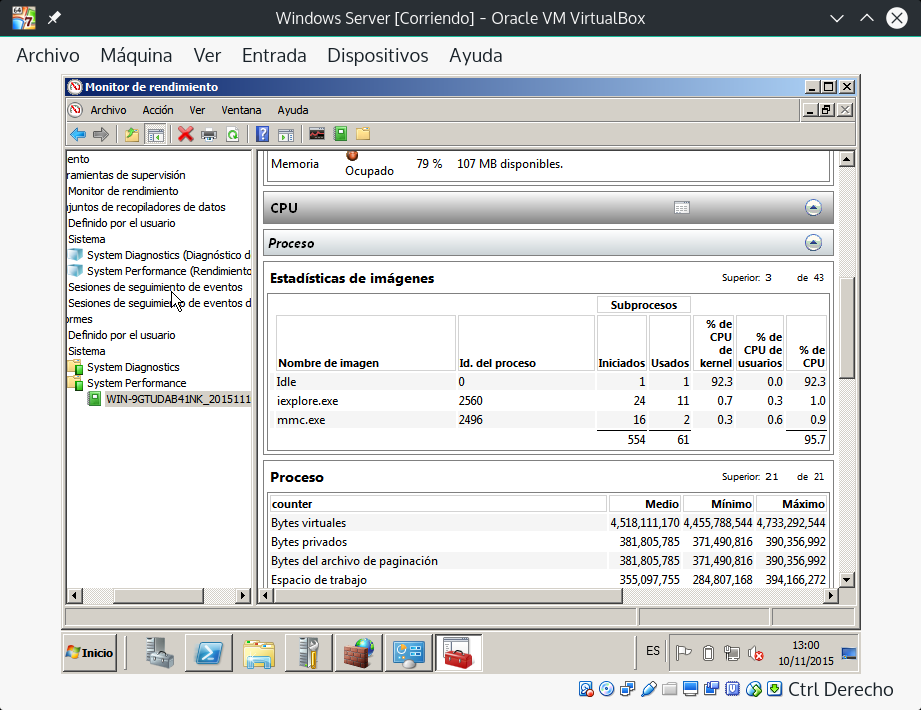
\includegraphics[scale=0.5]{figuras/figura7.png}  %el parámetro scale permite agrandar o achicar la imagen. En el nombre de archivo puede especificar directorios
	\label{figura7}
	
	\caption{Estadísticas de imágenes} 
\end{figure}

%%%%%%%%%%%%%%%%%%%%%%%%%%%%%%%%%%%%%%%%%%%%%%%%%%%%
% CUESTIÓN 5
%%%%%%%%%%%%%%%%%%%%%%%%%%%%%%%%%%%%%%%%%%%%%%%%%%%%

\section{Cuestión 5: Cree un recopilador de datos definido por el usuario (modo avanzado) que incluya tanto el contador de rendimiento como los datos deseguimiento: Todos los referentes al procesador, al proceso y al servicio web. Intervalo de muestra 15 segundos. Almacene el resultado en el directorio Escritorio\textbackslash logs. Incluya las capturas de pantalla de cada paso.}
\begin{figure}[H] %con el [H] le obligamos a situar aquí la figura
	\centering
	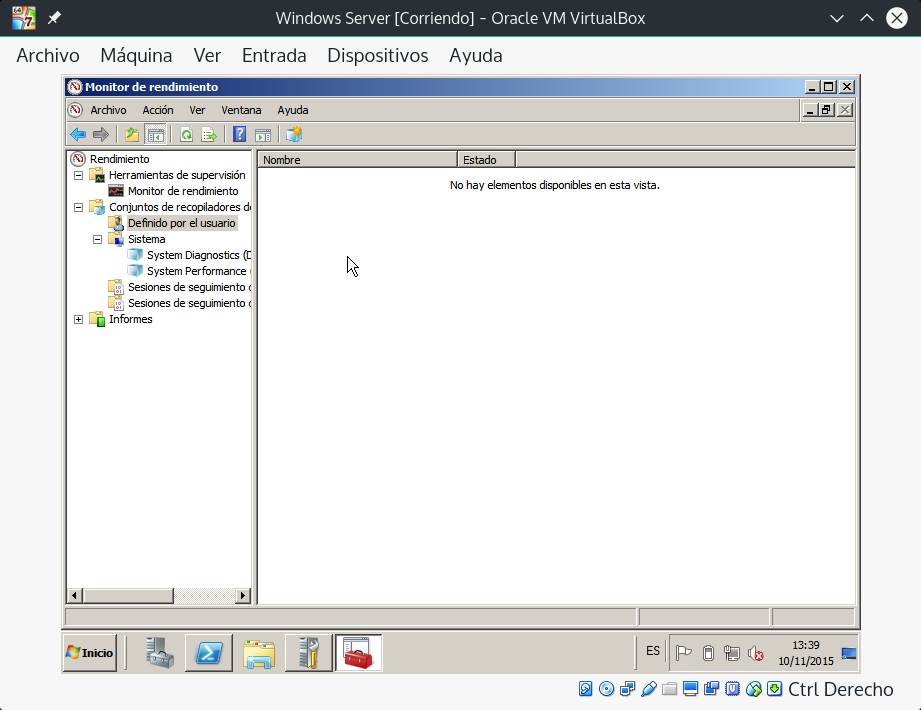
\includegraphics[scale=0.5]{figuras/figura10.png}  %el parámetro scale permite agrandar o achicar la imagen. En el nombre de archivo puede especificar directorios
	\label{figura10}
	
	\caption{Realizamos un click izquierdo en la carpeta Definido por el usuario} 
\end{figure}

\begin{figure}[H] %con el [H] le obligamos a situar aquí la figura
	\centering
	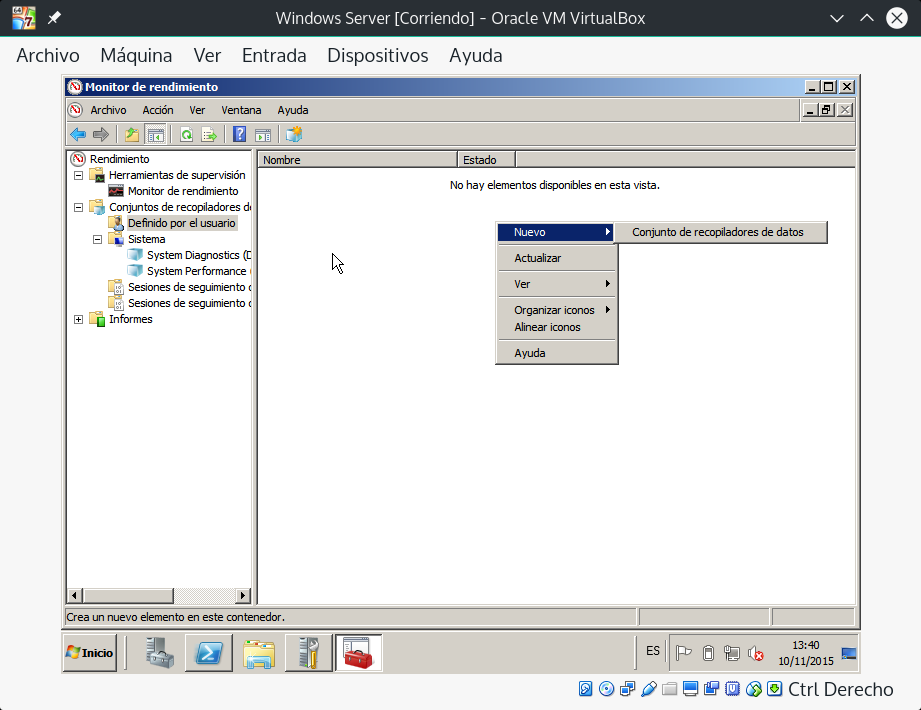
\includegraphics[scale=0.4]{figuras/figura11.png}  %el parámetro scale permite agrandar o achicar la imagen. En el nombre de archivo puede especificar directorios
	\label{figura11}
	
	\caption{Realizamos un click derecho y seleccionamos nuevo->conjunto de recopiladores de datos} 
\end{figure}

\begin{figure}[H] %con el [H] le obligamos a situar aquí la figura
	\centering
	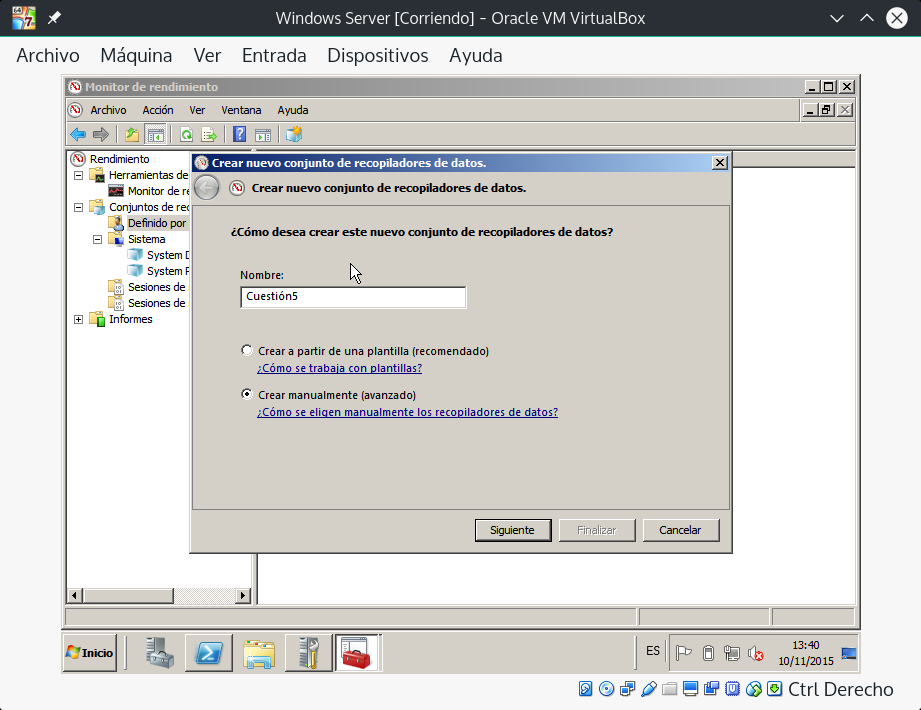
\includegraphics[scale=0.4]{figuras/figura12.png}  %el parámetro scale permite agrandar o achicar la imagen. En el nombre de archivo puede especificar directorios
	\label{figura12}
	
	\caption{Renombramos con el nombre que deseemos y elegimos la opción de crear manualmente(avanzado)} 
\end{figure}

\begin{figure}[H] %con el [H] le obligamos a situar aquí la figura
	\centering
	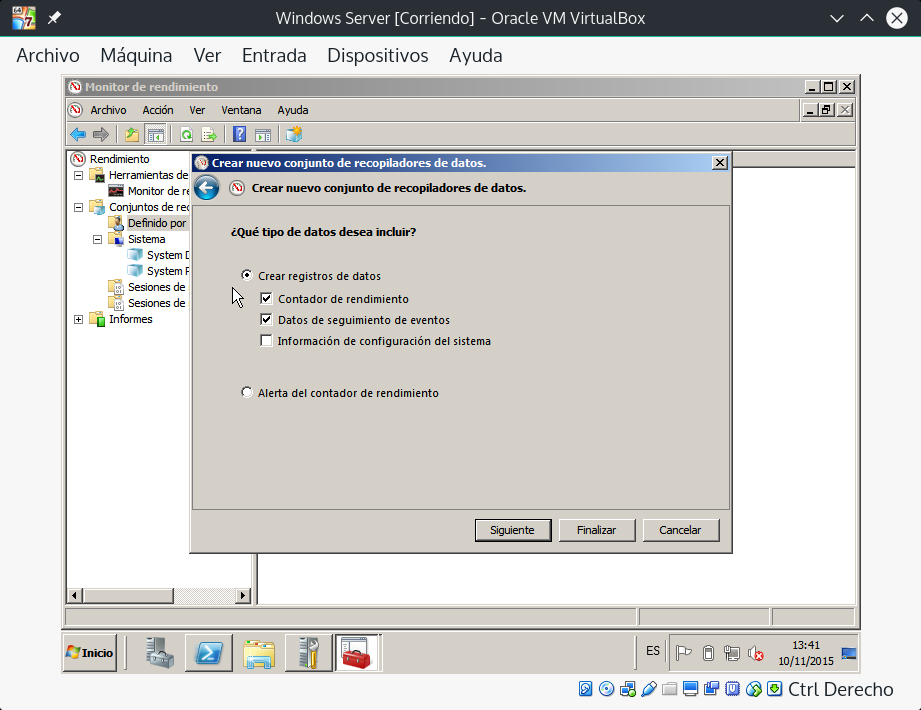
\includegraphics[scale=0.4]{figuras/figura13.png}  %el parámetro scale permite agrandar o achicar la imagen. En el nombre de archivo puede especificar directorios
	\label{figura13}
	
	\caption{Elegimos la opción de crear registros de datos y pulsamos para seleccionar las opciones de: \textbf{Contador de rendimiento} y \textbf{Datos de seguimiento de eventos}} 
\end{figure}
\begin{figure}[H] %con el [H] le obligamos a situar aquí la figura
	\centering
	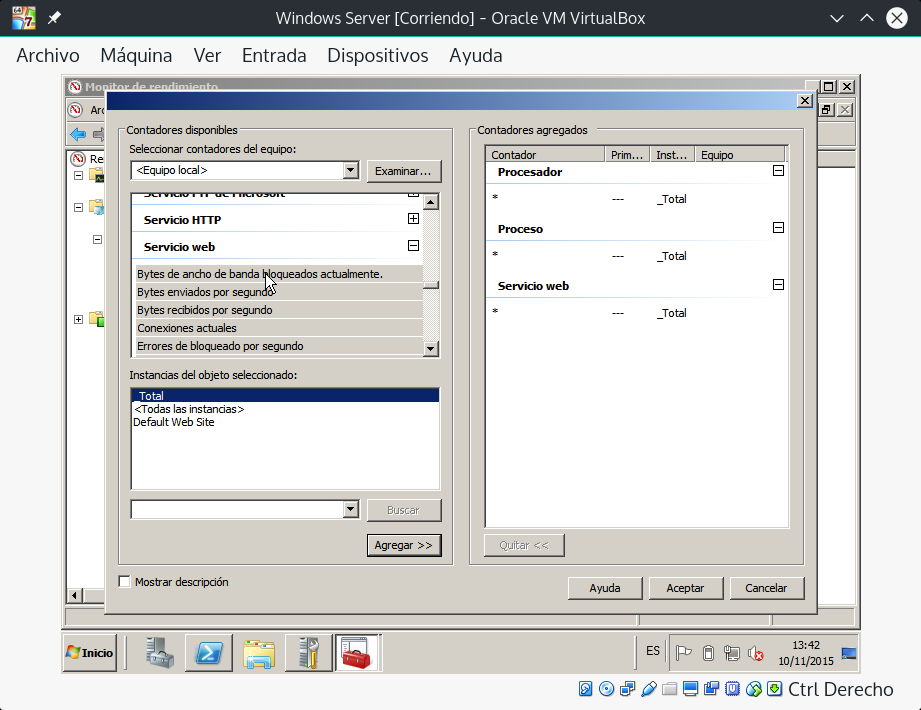
\includegraphics[scale=0.4]{figuras/figura14.png}  %el parámetro scale permite agrandar o achicar la imagen. En el nombre de archivo puede especificar directorios
	\label{figura14}
	
	\caption{Pulsamos sobre \textbf{Procesador, Proceso y Servicios Web} y nos selecciona todo lo que hay dentro de ellos. Una vez seleccionados le damos a Agregar.} 
\end{figure}

\begin{figure}[H] %con el [H] le obligamos a situar aquí la figura
	\centering
	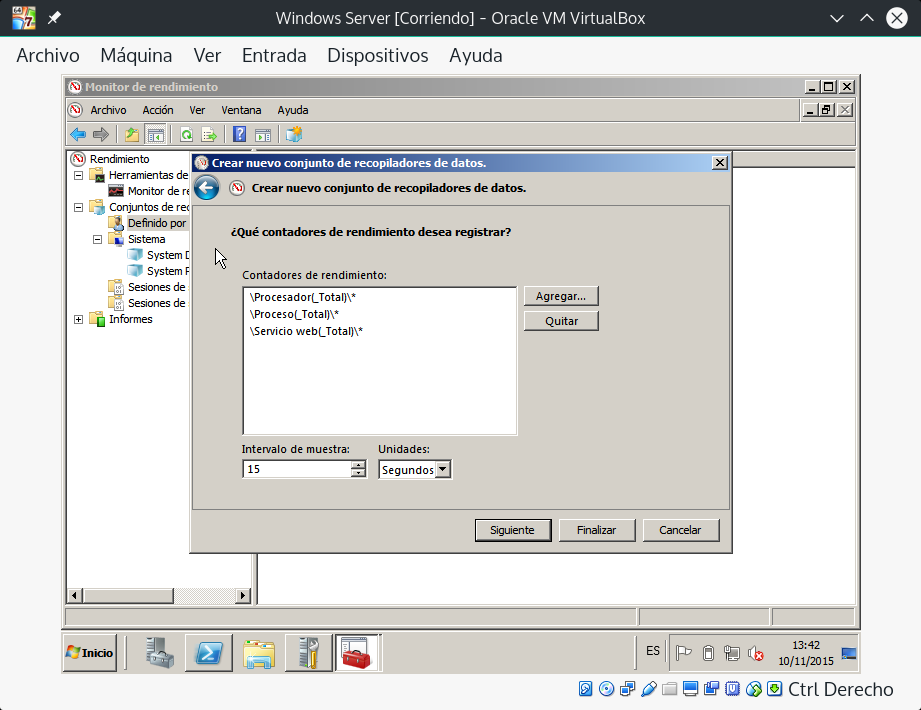
\includegraphics[scale=0.4]{figuras/figura15.png}  %el parámetro scale permite agrandar o achicar la imagen. En el nombre de archivo puede especificar directorios
	\label{figura15}
	
	\caption{Aquí por defecto nos viene el Intervalo de muestreo 15 segundos, por lo que solo le debemos dar a siguiente.} 
\end{figure}
\begin{figure}[H] %con el [H] le obligamos a situar aquí la figura
	\centering
	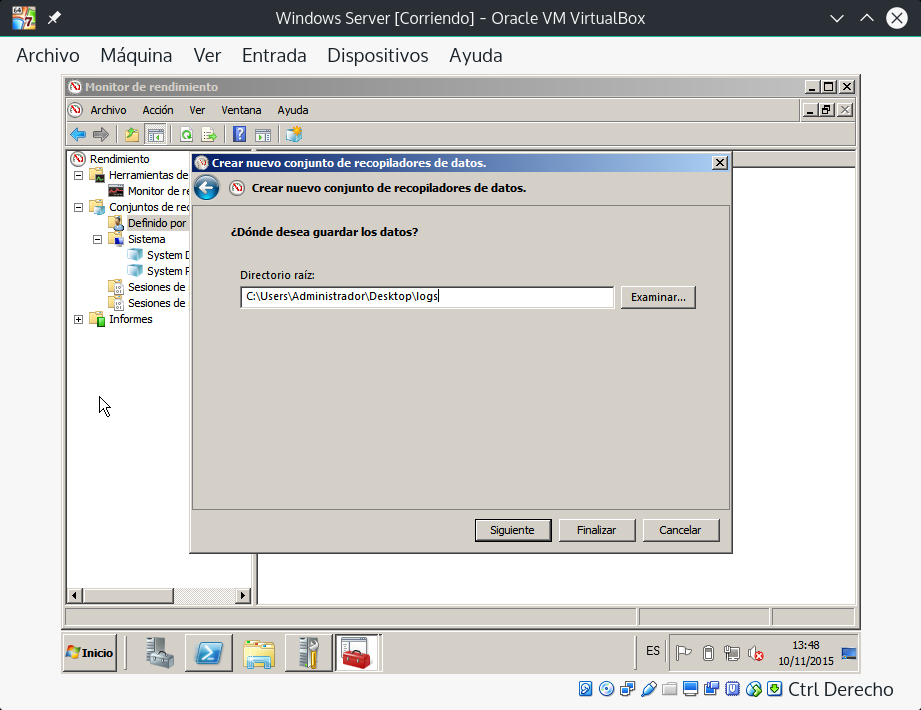
\includegraphics[scale=0.4]{figuras/figura16.png}  %el parámetro scale permite agrandar o achicar la imagen. En el nombre de archivo puede especificar directorios
	\label{figura16}
	
	\caption{Aquí elegimos donde se van a guardar los log generados, en nuestro caso será en Escritorio/logs} 
\end{figure}
\begin{figure}[H] %con el [H] le obligamos a situar aquí la figura
	\centering
	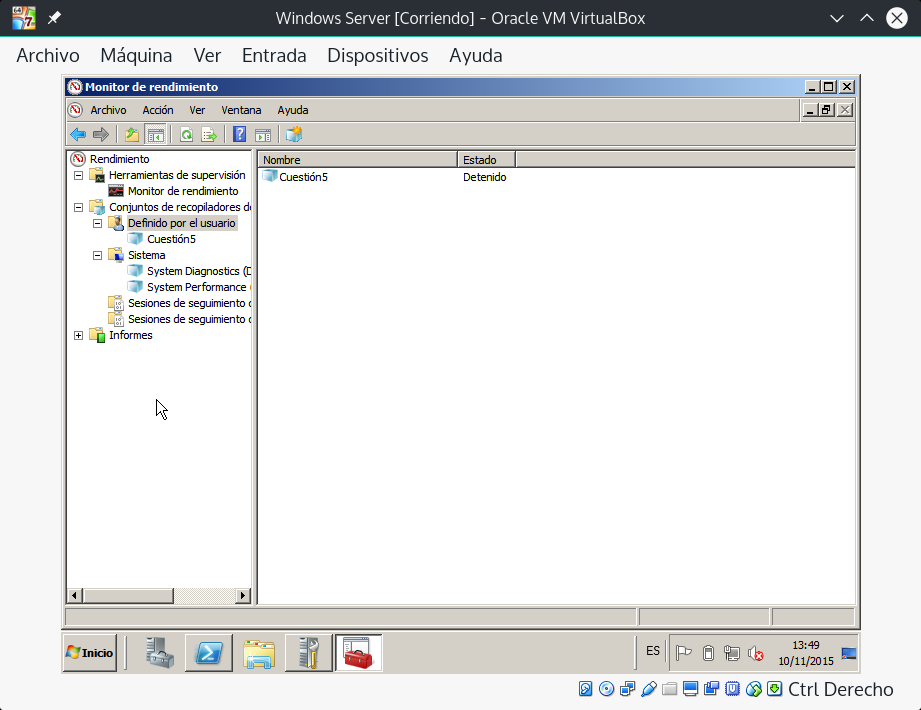
\includegraphics[scale=0.4]{figuras/figura17.png}  %el parámetro scale permite agrandar o achicar la imagen. En el nombre de archivo puede especificar directorios
	\label{figura17}
	
	\caption{Podemos observar como se ha creado} 
\end{figure}
\begin{figure}[H] %con el [H] le obligamos a situar aquí la figura
	\centering
	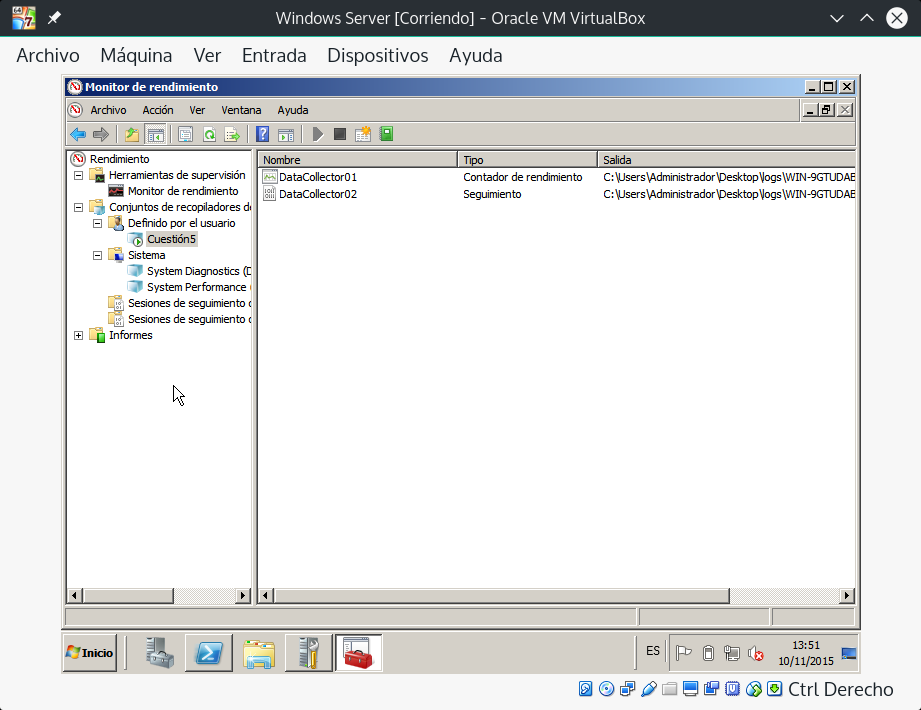
\includegraphics[scale=0.4]{figuras/figura18.png}  %el parámetro scale permite agrandar o achicar la imagen. En el nombre de archivo puede especificar directorios
	\label{figura18}
	
	\caption{Realizamos un click con el botón derecho y le damos a iniciar} 
\end{figure}
\begin{figure}[H] %con el [H] le obligamos a situar aquí la figura
	\centering
	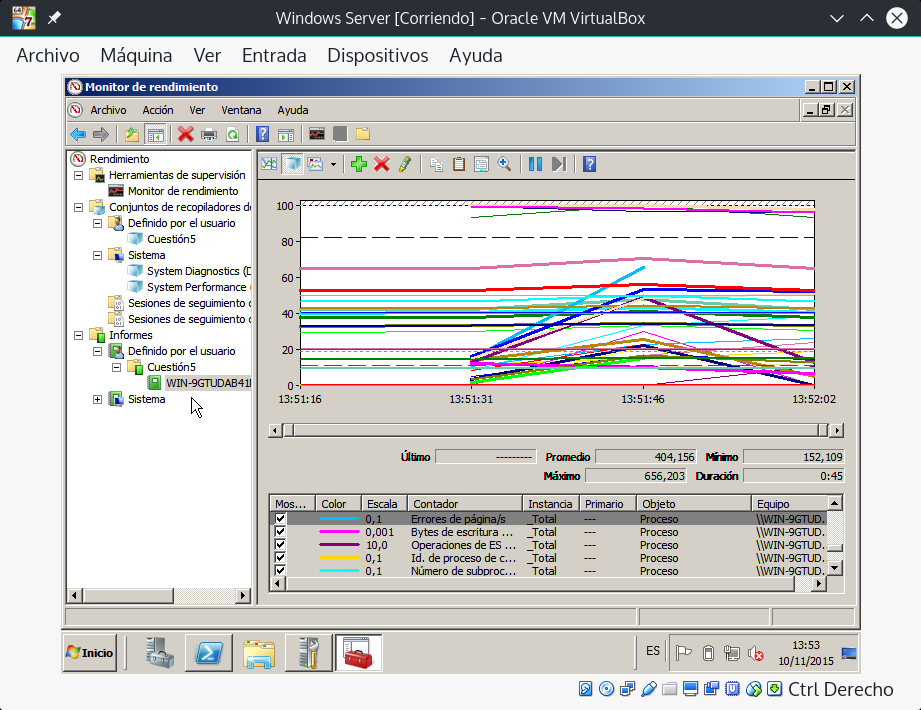
\includegraphics[scale=0.4]{figuras/figura19.png}  %el parámetro scale permite agrandar o achicar la imagen. En el nombre de archivo puede especificar directorios
	\label{figura19}
	
	\caption{Imagen con el resultado del monitor} 
\end{figure}
Vamos a analizar los resultados que hemos obtenido de la monitorización:\\
Lo primero es que el tiempo de monitorización ha sido escaso para poder analizar los datos de unas acciones determinadas, las cuáles han sido el inicio de las aplicaciones Internet Explorer y Notepad, y que no se viera afectado por otrod datos que se dieran en la máquina virtual.\\
Podemos observar en la gráfica que entre las \textbf{13:51:16} y las \textbf{13:51:31} todo se mantiene estable, ya que durante este tiempo dejé la máquina virtual en reposo sin realizar ninguna acción.\\
A partir de las \textbf{13:51:31} fué cuando ejecuté las aplicaciones Internet Explorer y Notepad. Podemos comproba el uso  NotePad ya que en la Figura 5.10 se ve las \textcolor{azuloscuro}{Operaciones E/S de datos} va creciendo hasta que se puede observa el pico máximo a las \textbf{13:51:56}, momento en el que se cierra la aplicación y comienza a bajar. Lo mismo ocurre con el uso de Internet Explorer, podemos observar con \textcolor{rosa}{Nº Total de Intentos de conexión} que comienza  a las \textbf{13:51:31} y va decreciendo hasta el final.\\
Después de alcanzar el piso a las \textbf{13:51:46} descienden la mayoría de valores hasta que termina la monitorización a las \textbf{13:52:02}. 
%%%%%%%%%%%%%%%%%%%%%%%%%%%%%%%%%%%%%%%%%%%%%%%%%%%%
% CUESTIÓN 6
%%%%%%%%%%%%%%%%%%%%%%%%%%%%%%%%%%%%%%%%%%%%%%%%%%%%

\section{Cuestión 6: instale alguno de los monitores comentados arriba en su máquina y pruebe a ejecutarlos (tenga en cuenta que si lo hace en la máquina virtual, los resultados pueden no ser realistas). Alternativamente, busque otros monitores para hardware comerciales o de código abierto para Windows y Linux.}
Vamos a probar el monitor 	\textbf{hddtemp}.\\
Con el comando \textbf{sudo fdisk -l} podemos ver todos los discos duros montados en nuestra máquina junto con sus particiones y al información de las mismas.

\begin{figure}[H] %con el [H] le obligamos a situar aquí la figura
	\centering
	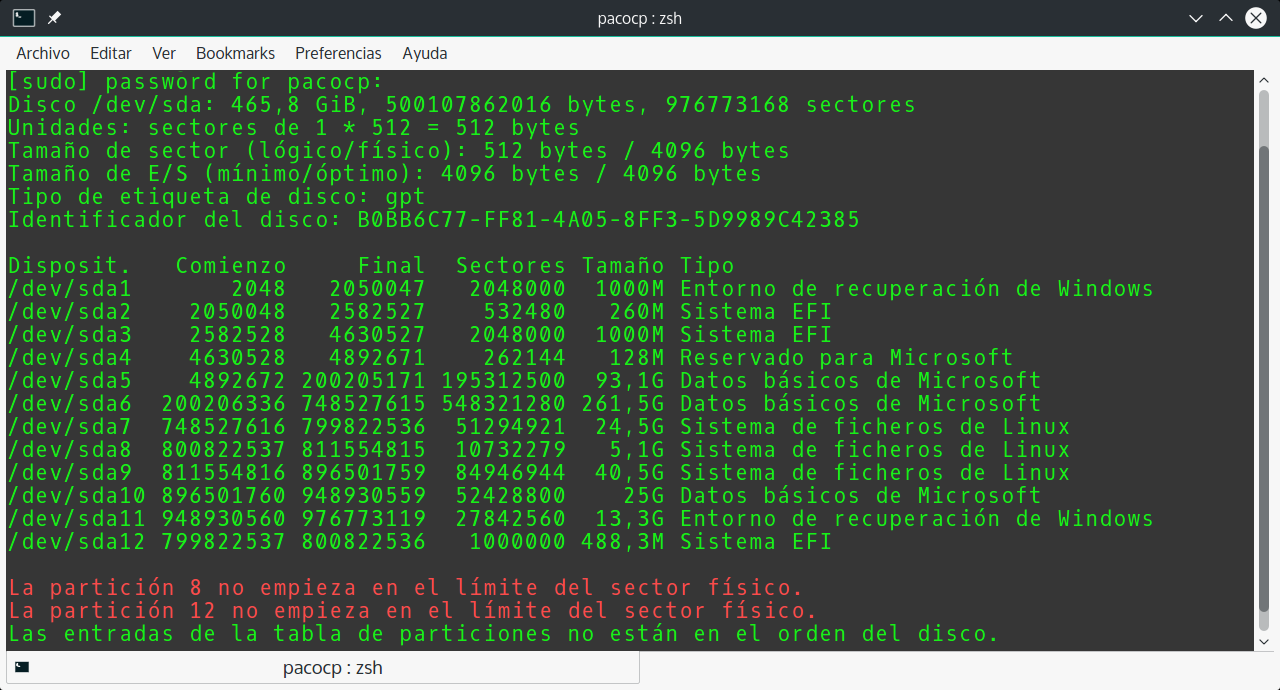
\includegraphics[scale=0.4]{figuras/figura20.png}  %el parámetro scale permite agrandar o achicar la imagen. En el nombre de archivo puede especificar directorios
	\label{figura20}
	
	\caption{Podemos observar el disco junto con sus particiones existentes} 
\end{figure}

Para ver la temperatura de ese disco utilizamos el comando: \textbf{sudo hddtemp /dev/sda}

\begin{figure}[H] %con el [H] le obligamos a situar aquí la figura
	\centering
	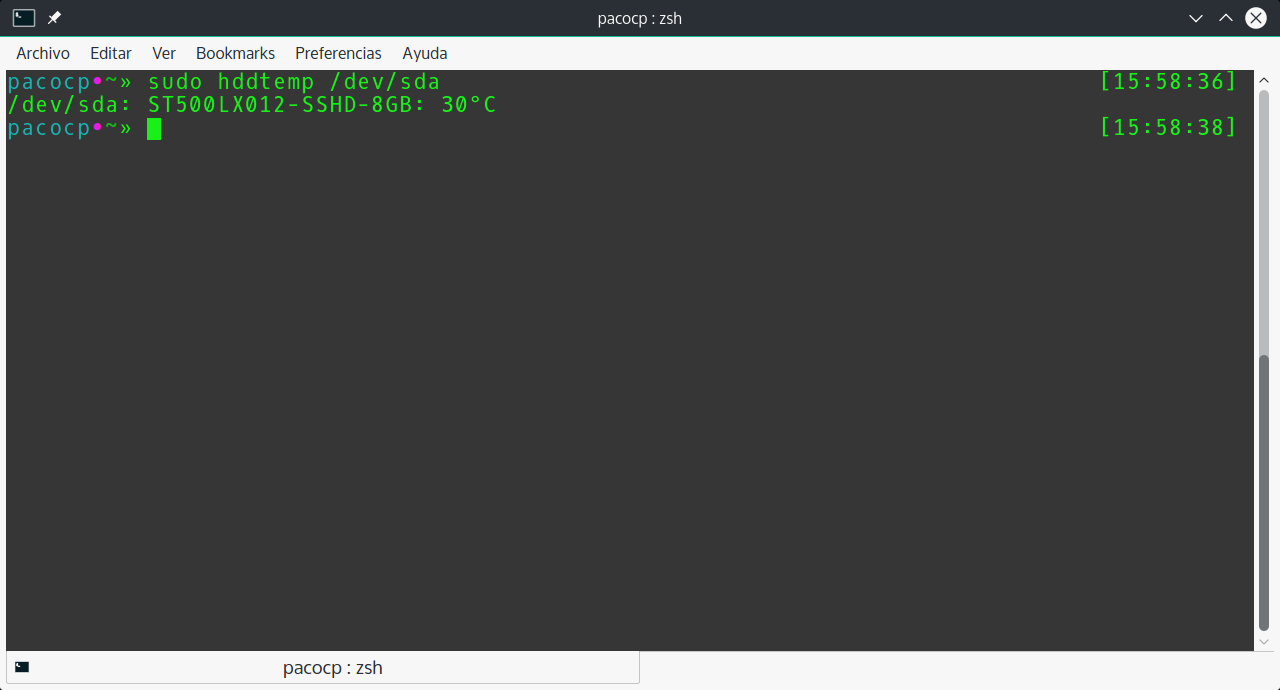
\includegraphics[scale=0.4]{figuras/figura21.png}  %el parámetro scale permite agrandar o achicar la imagen. En el nombre de archivo puede especificar directorios
	\label{figura21}
	
	\caption{Nos dice la temperatura del disco} 
\end{figure}

La temperatura que obtener es de 30 grados centígrados que ,según múltiples referencias \cite{hddt} \cite{hddt2}, se encuentra en el intervalo de temperatura adecuado para un HDD.\\

Algunos monitores tanto para Windows como para Linux serían:
\begin{itemize}
	\item \textbf{HWMonitor\cite{hwm}: } Disponible  para Windows 
	\item \textbf{Hardware Sensors Monitor \cite{hsm}: } Disponible para Windows
\end{itemize}

%%%%%%%%%%%%%%%%%%%%%%%%%%%%%%%%%%%%%%%%%%%%%%%%%%%%
% CUESTIÓN 7
%%%%%%%%%%%%%%%%%%%%%%%%%%%%%%%%%%%%%%%%%%%%%%%%%%%%

\section{Cuestión 7: Visite la web del proyecto y acceda a la demo que proporcionan (http://demo.munin-monitoring.org/) donde se muestra cómo monitorizan un servidor. Monitorice varios parámetros y haga capturas de pantalla de lo que está mostrando comentando qué observa.}
\begin{figure}[H] %con el [H] le obligamos a situar aquí la figura
	\centering
	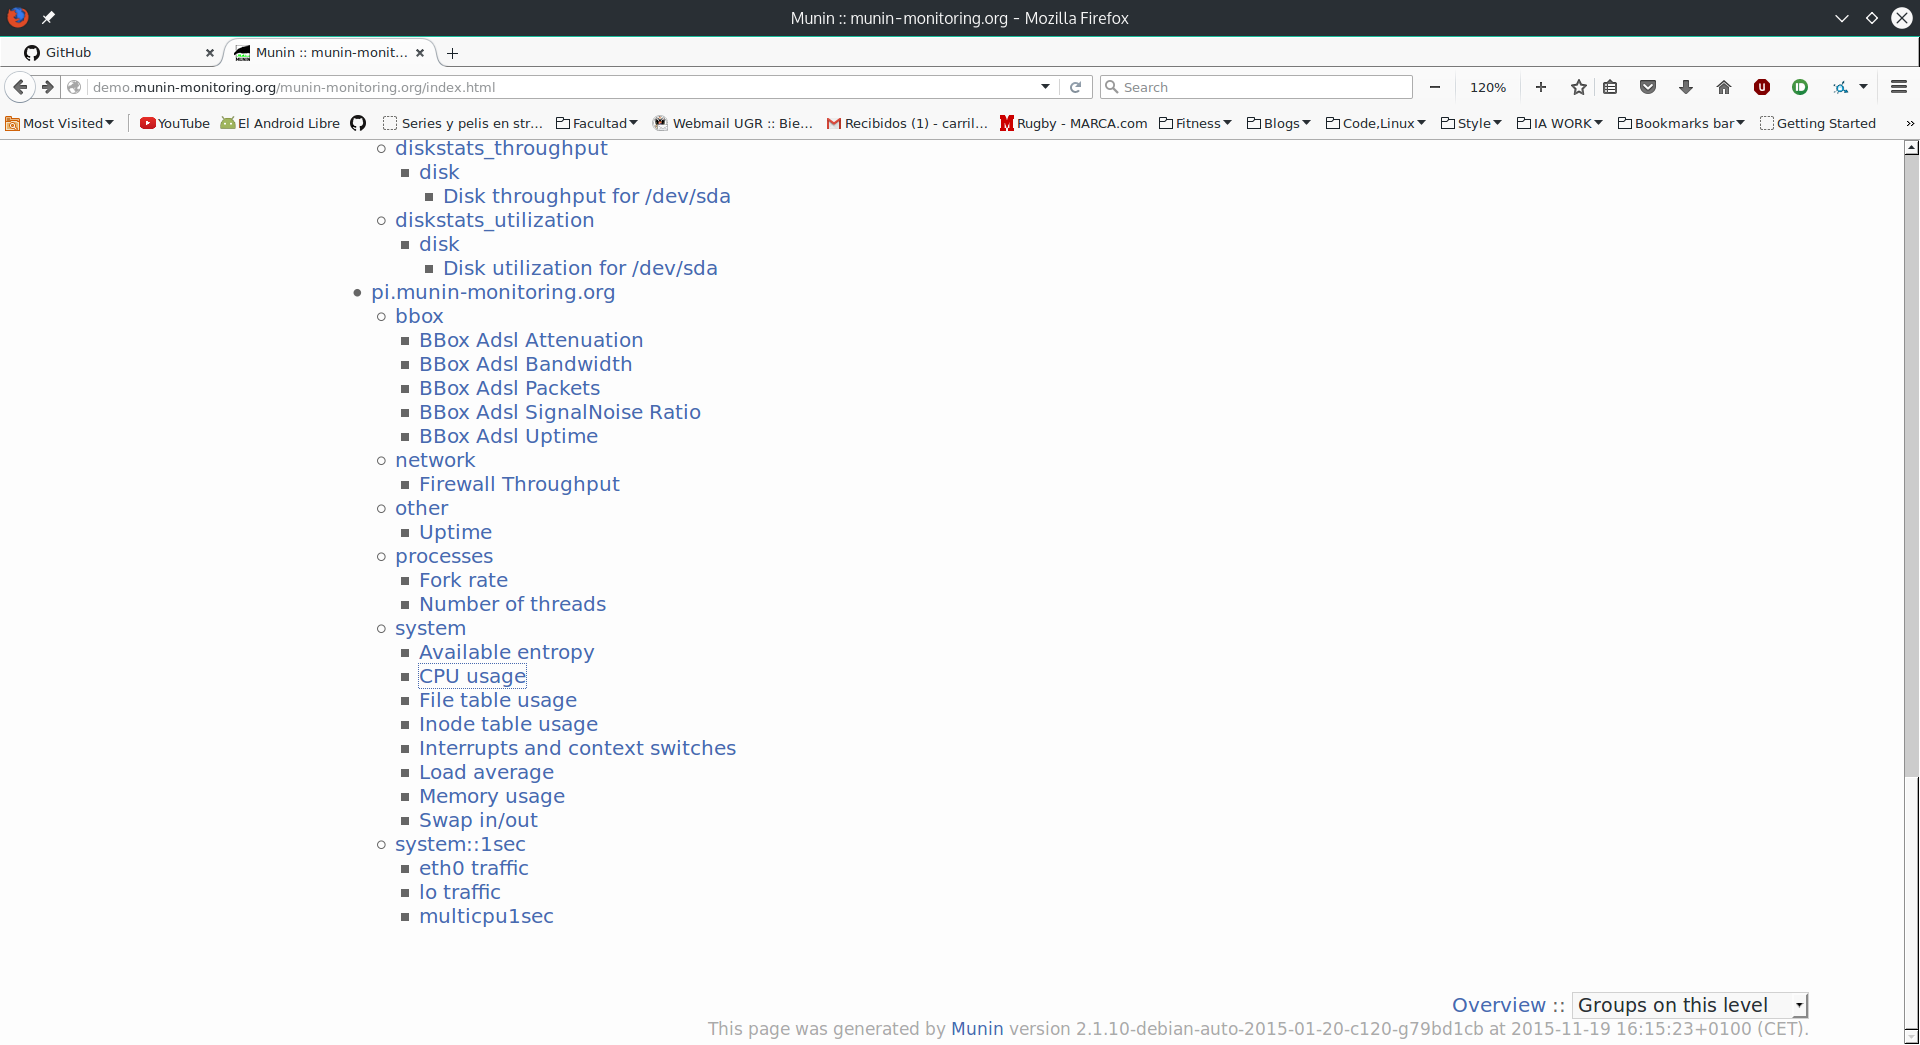
\includegraphics[scale=0.25]{figuras/figura22.png}  %el parámetro scale permite agrandar o achicar la imagen. En el nombre de archivo puede especificar directorios
	\label{figura22}
	
	\caption{En primer lugar vamos a monitorizar la CPU} 
\end{figure}
\begin{figure}[H] %con el [H] le obligamos a situar aquí la figura
	\centering
	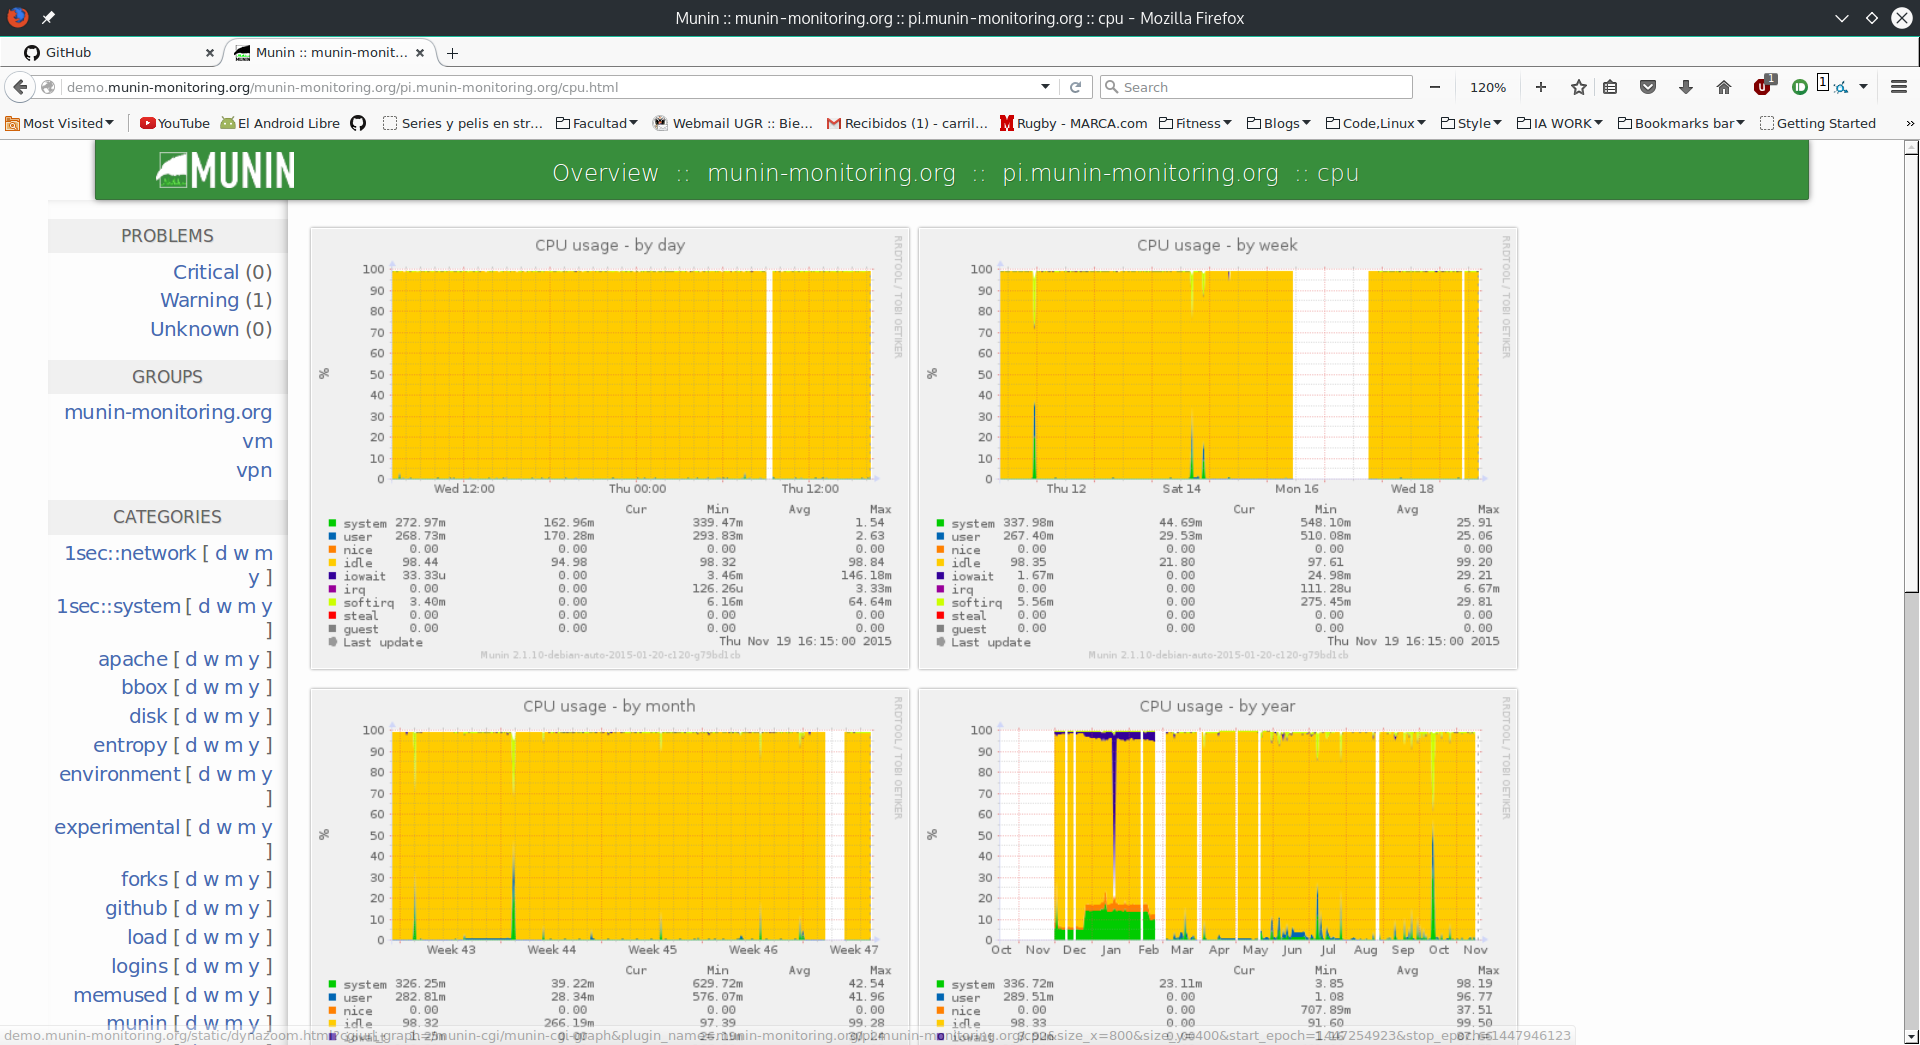
\includegraphics[scale=0.25]{figuras/figura23.png}  %el parámetro scale permite agrandar o achicar la imagen. En el nombre de archivo puede especificar directorios
	\label{figura23}
	
	\caption{Aquí podemos observar los distintos tipos de monitorización, por escala de tiempo, por día, por semana, por mes o por año.} 
\end{figure}

Si nos fijamos en la Figura 7.2 podemos observar el uso de la CPU en un día. En este caso los datos que nos muestra son:
\begin{itemize}
	\item \textcolor{verde}{system}
	\item \textcolor{azuloscuro}{user}
	\item \textcolor{naranja}{nice}
	\item \textcolor{amarillo}{idle}
	\item \textcolor{morado}{iowait}
	\item \textcolor{violeta}{irq}
	\item \textcolor{verdelima}{softirq}
	\item \textcolor{rojo}{steal}
	\item \textcolor{gris}{guest}
\end{itemize}
\begin{figure}[H] %con el [H] le obligamos a situar aquí la figura
	\centering
	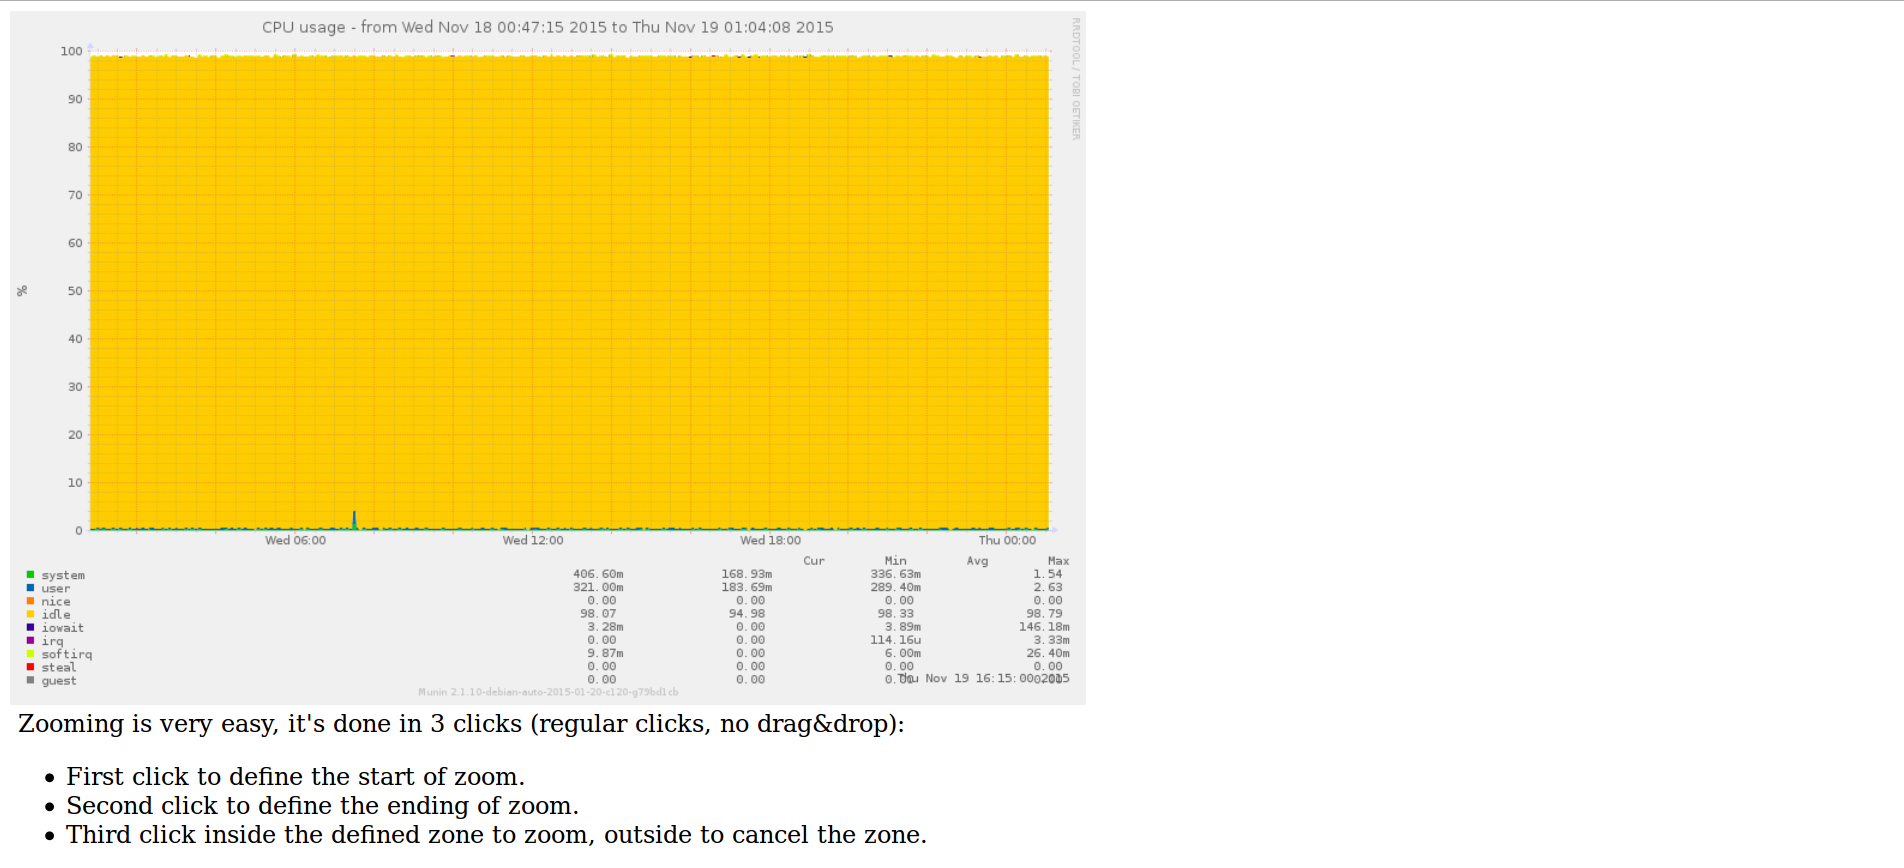
\includegraphics[scale=0.25]{figuras/figura24.png}  %el parámetro scale permite agrandar o achicar la imagen. En el nombre de archivo puede especificar directorios
	\label{figura24}
	
	\caption{Opción de monitorización por día} 
\end{figure}

Si nos fijamos el los picos podemos observar que ambos se deben a uso de la CPU por parte de  \textcolor{verde}{system} y \textcolor{azuloscuro}{user}, que ambos son los que más uso hacen de la CPU como se puede observar en las estadísticas inferiores a la imagen.
\\
Ahora por ejemplo podríamos monitorizar el uso de las distintas CPU.

\begin{figure}[H] %con el [H] le obligamos a situar aquí la figura
	\centering
	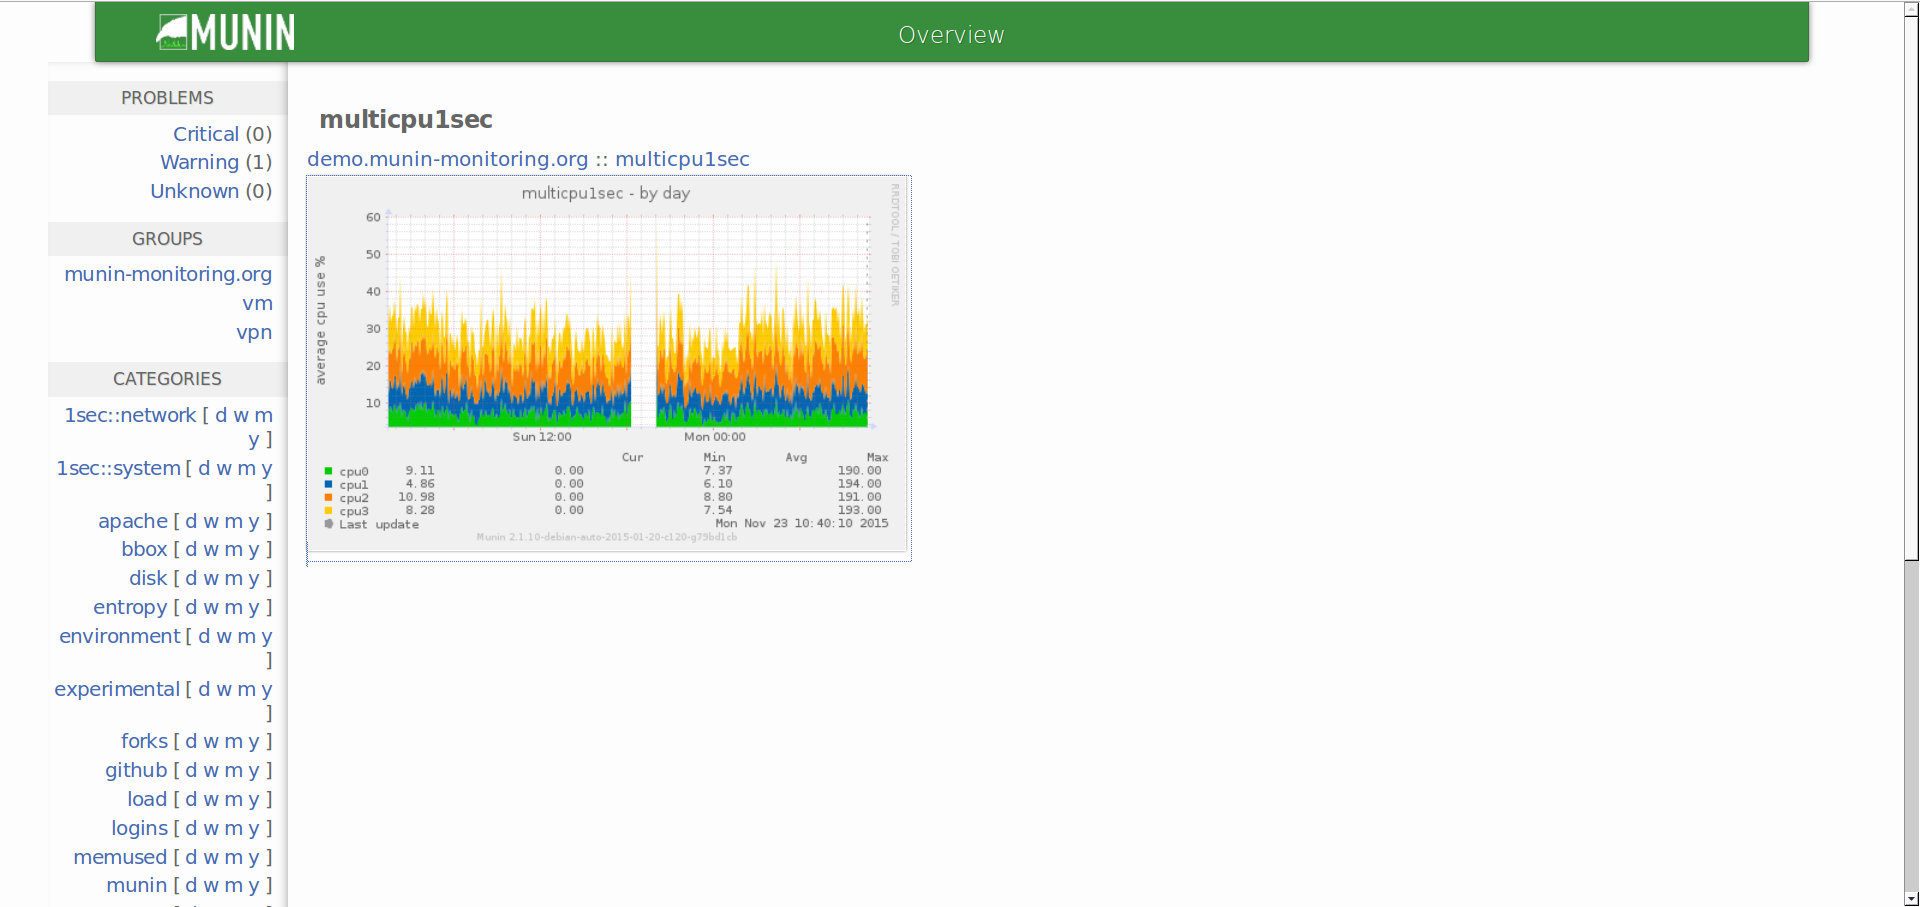
\includegraphics[scale=0.25]{figuras/figura37.png}  %el parámetro scale permite agrandar o achicar la imagen. En el nombre de archivo puede especificar directorios
	\label{figura37}
	
	\caption{Pulsamos para poder elegir entre los datos de monitorización por día,semana,mes...} 
\end{figure}

Una vez dentro podemos observar la gráfica en la Figura 7.5  las distintas CPU y su uso:\\

\begin{itemize}
	\item \textcolor{verde}{cpu0} : podemos observar que no es la que tiene menos uso pero es la que no alcanza grandes máximos en su uso.
	\item \textcolor{azuloscuro}{cpu1} : es la que menos se usa con 5.44 , pero tiene valores más altos que \textcolor{verde}{cpu0} siendo su mínimo 6.07 y su máximo 194.00 siendo este el valor más alto de la gráfica.
	\item \textcolor{naranja}{cpu2} : es la que más se usa con 15.18, siendo su mínimo 8.81 y su máximo 191.0
	\item \textcolor{amarillo}{cpu3} es la última siendo su valor mínimo 7.48 y su máximo 198.0
\end{itemize}

\begin{figure}[H] %con el [H] le obligamos a situar aquí la figura
	\centering
	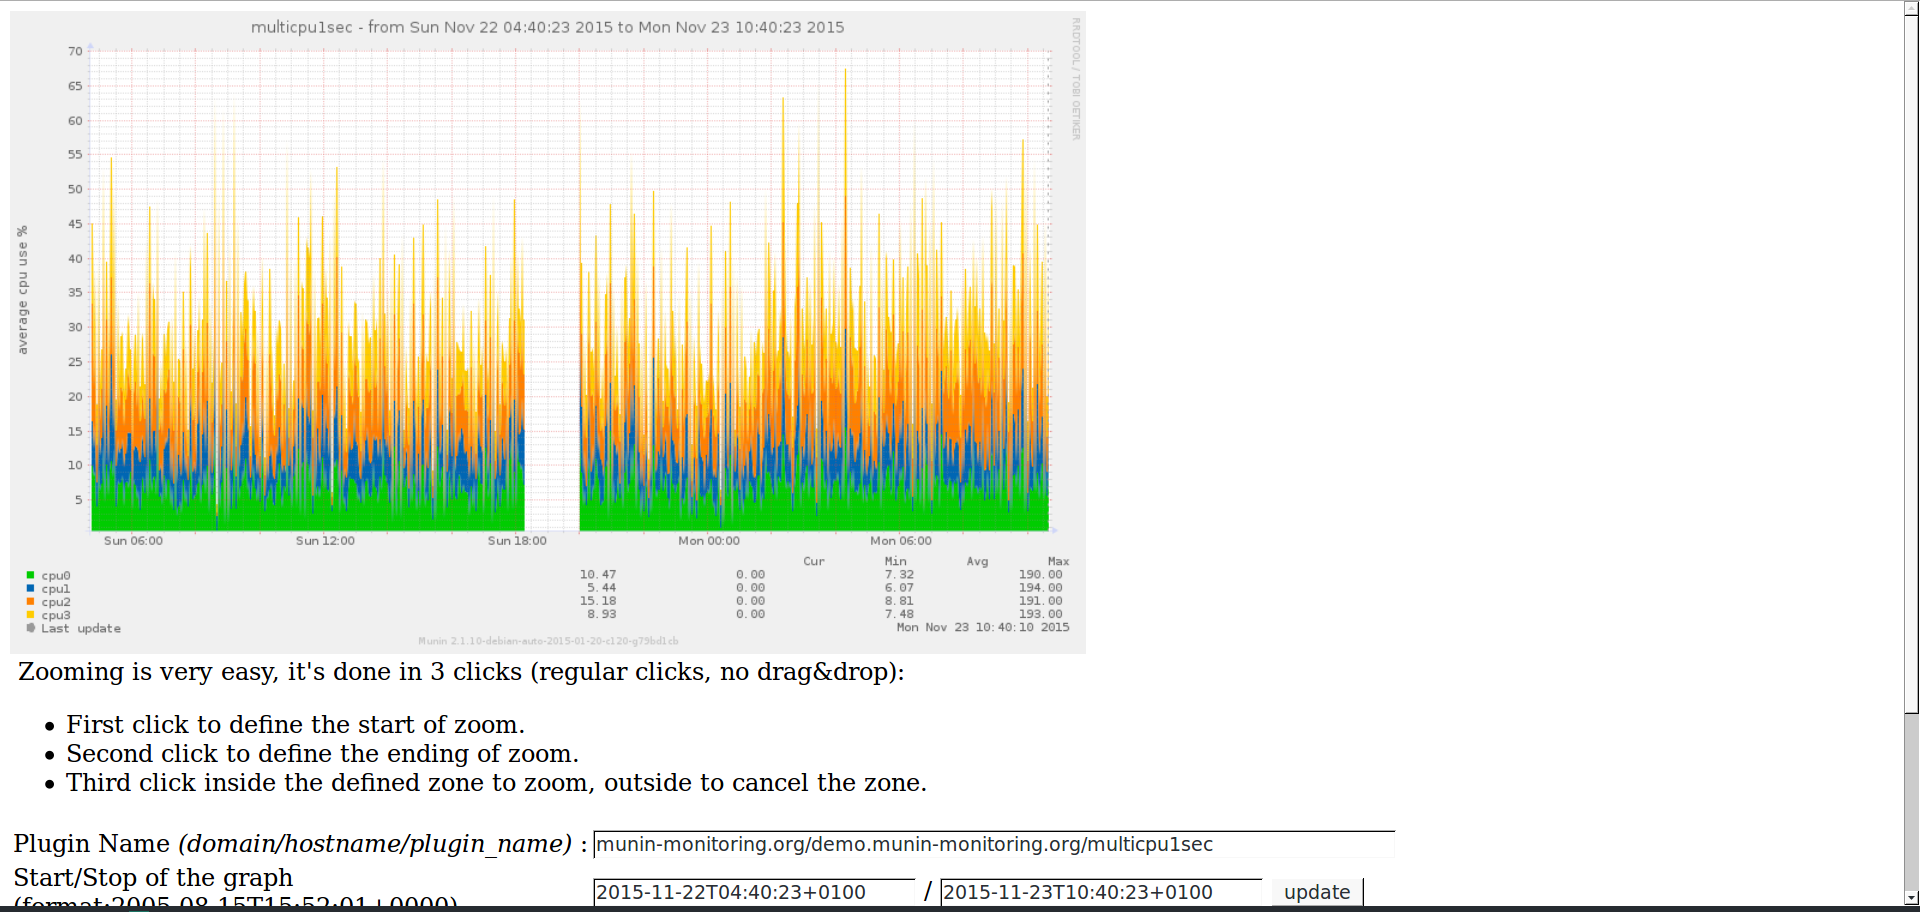
\includegraphics[scale=0.25]{figuras/figura38.png}  %el parámetro scale permite agrandar o achicar la imagen. En el nombre de archivo puede especificar directorios
	\label{figura38}
	
	\caption{Monitorización del sistema por día} 
\end{figure}
%%%%%%%%%%%%%%%%%%%%%%%%%%%%%%%%%%%%%%%%%%%%%%%%%%%%
% CUESTIÓN 8
%%%%%%%%%%%%%%%%%%%%%%%%%%%%%%%%%%%%%%%%%%%%%%%%%%%%

\section{Cuestión 8: Escriba un breve resumen sobre alguno de los artículos donde se muestra el uso de strace o busque otro y coméntelo.}

Leyendo el artículo \cite{strace} podemos observar lo útil que puede ser seguir la traza de ejecución de un programa. El autor del mismo, Steven Kemp, nos cuenta como gracias a esta utilidad pudo resolver un problema con un servidor SVN que no se comportaba correctamente. Gracias al comando \textbf{strace} podemos observar toda la traza de un programa en ejecución por ejemplo, todas las llamadas al sistema que va realizando. Un ejemplo serían las llamadas de open a archivos que va realizando el programa.\\
En su caso los problemas con el servidor eran:\\

\begin{itemize}
	\item \textquotedblleft Un servidor SVN que fue configurado en el pasado.\textquotedblright
	\item \textquotedblleft Los clientes que utilizaban Microsoft Windows podían conectarse al servidor mediante un cliente SVN \textquotedblright
	\item \textquotedblleft En algún momento algunos clientes se  colgaban  y una vez que se habían colgado nadie podía acceder al servidor SVN \textquotedblright
	\item \textquotedblleft Reiniciar el servidor arreglaba el problema temporalmente \textquotedblright
\end{itemize}

Al principio intentó mirar los archivos log, pero no existía ninguno.\\
Entonces creó un script que ejecutara el binario para comprobar en que momento se colgaba. Al hacerlo pudo observar que se producía un problema con la llamada para abrir un fichero: \textbf{/dev/random} \\
Los clientes abrían este fichero para leer un número aleatorio de números y la apertura funcionaba, el problema estaba en la lectura. Como indica el artículo: \textquotedblleft Se podía ver que la lectura fallaba ya que la llamada de lectura se quedaba a medias \textquotedblright \\
El programa \textbf{/dev/random} se paraba si no había suficiente espacio para generar el flujo de datos. Por ello era por lo que reiniciar el servidor arreglaba el problema, ya que se vaciaba.\\

Arregló este problema creando un link de \textbf{/dev/random} a  \textbf{/dev/urandom} que no se para cuando no hay suficiente espacio.\\

Por último, da unas observaciones finales de que hubiera sido casi imposible resolver este problema sin utilizar la utilidad \textbf{strace}.

%%%%%%%%%%%%%%%%%%%%%%%%%%%%%%%%%%%%%%%%%%%%%%%%%%%%
% CUESTIÓN 9
%%%%%%%%%%%%%%%%%%%%%%%%%%%%%%%%%%%%%%%%%%%%%%%%%%%%

\section{Cuestión 9: Acceda a la consola mysql (o a través de phpMyAdmin) y muestre el resultado de mostrar el ”profile” de una consulta (la creación de la BD y la consulta la puede hacer líbremente).}
\begin{figure}[H] %con el [H] le obligamos a situar aquí la figura
	\centering
	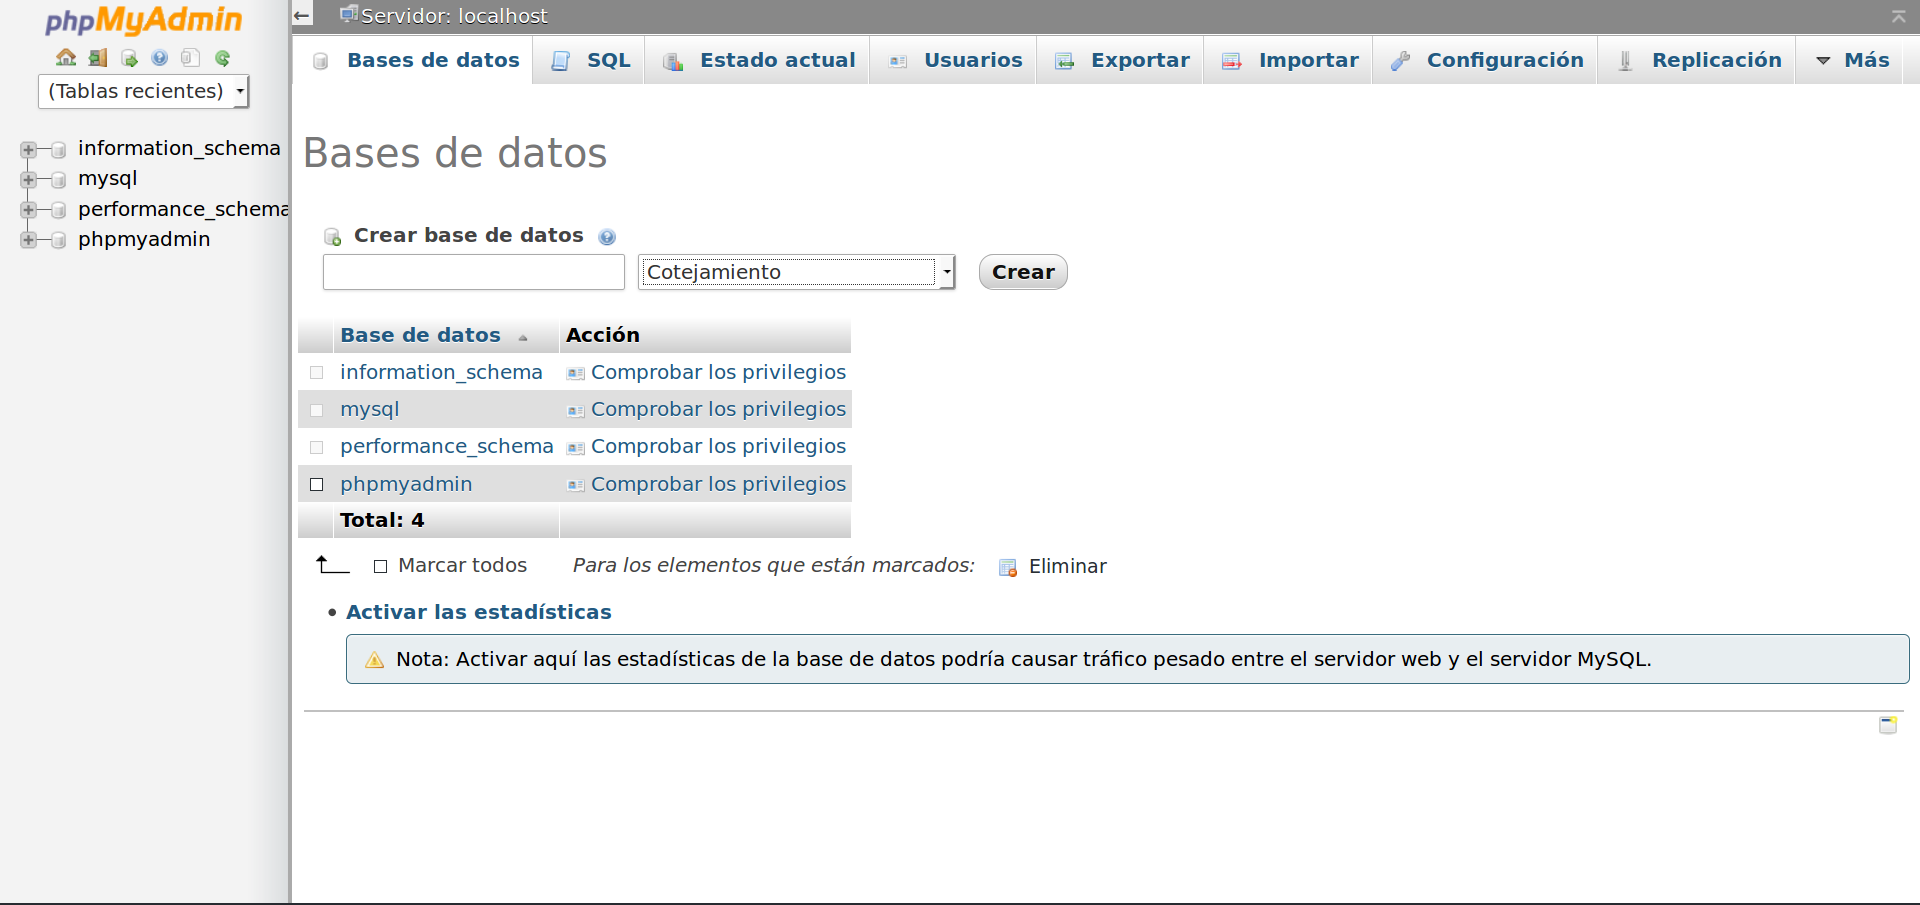
\includegraphics[scale=0.25]{figuras/figura25.png}  %el parámetro scale permite agrandar o achicar la imagen. En el nombre de archivo puede especificar directorios
	\label{figura25}
	
	\caption{Creación de la base de datos} 
\end{figure}

\begin{figure}[H] %con el [H] le obligamos a situar aquí la figura
	\centering
	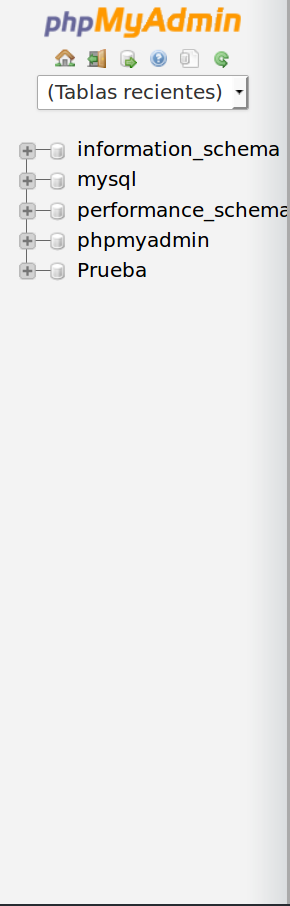
\includegraphics[scale=0.26]{figuras/figura26.png}  %el parámetro scale permite agrandar o achicar la imagen. En el nombre de archivo puede especificar directorios
	\label{figura26}
	
	\caption{Podemos observar como se ha creado la base de datos prueba} 
\end{figure}

\begin{figure}[H] %con el [H] le obligamos a situar aquí la figura
	\centering
	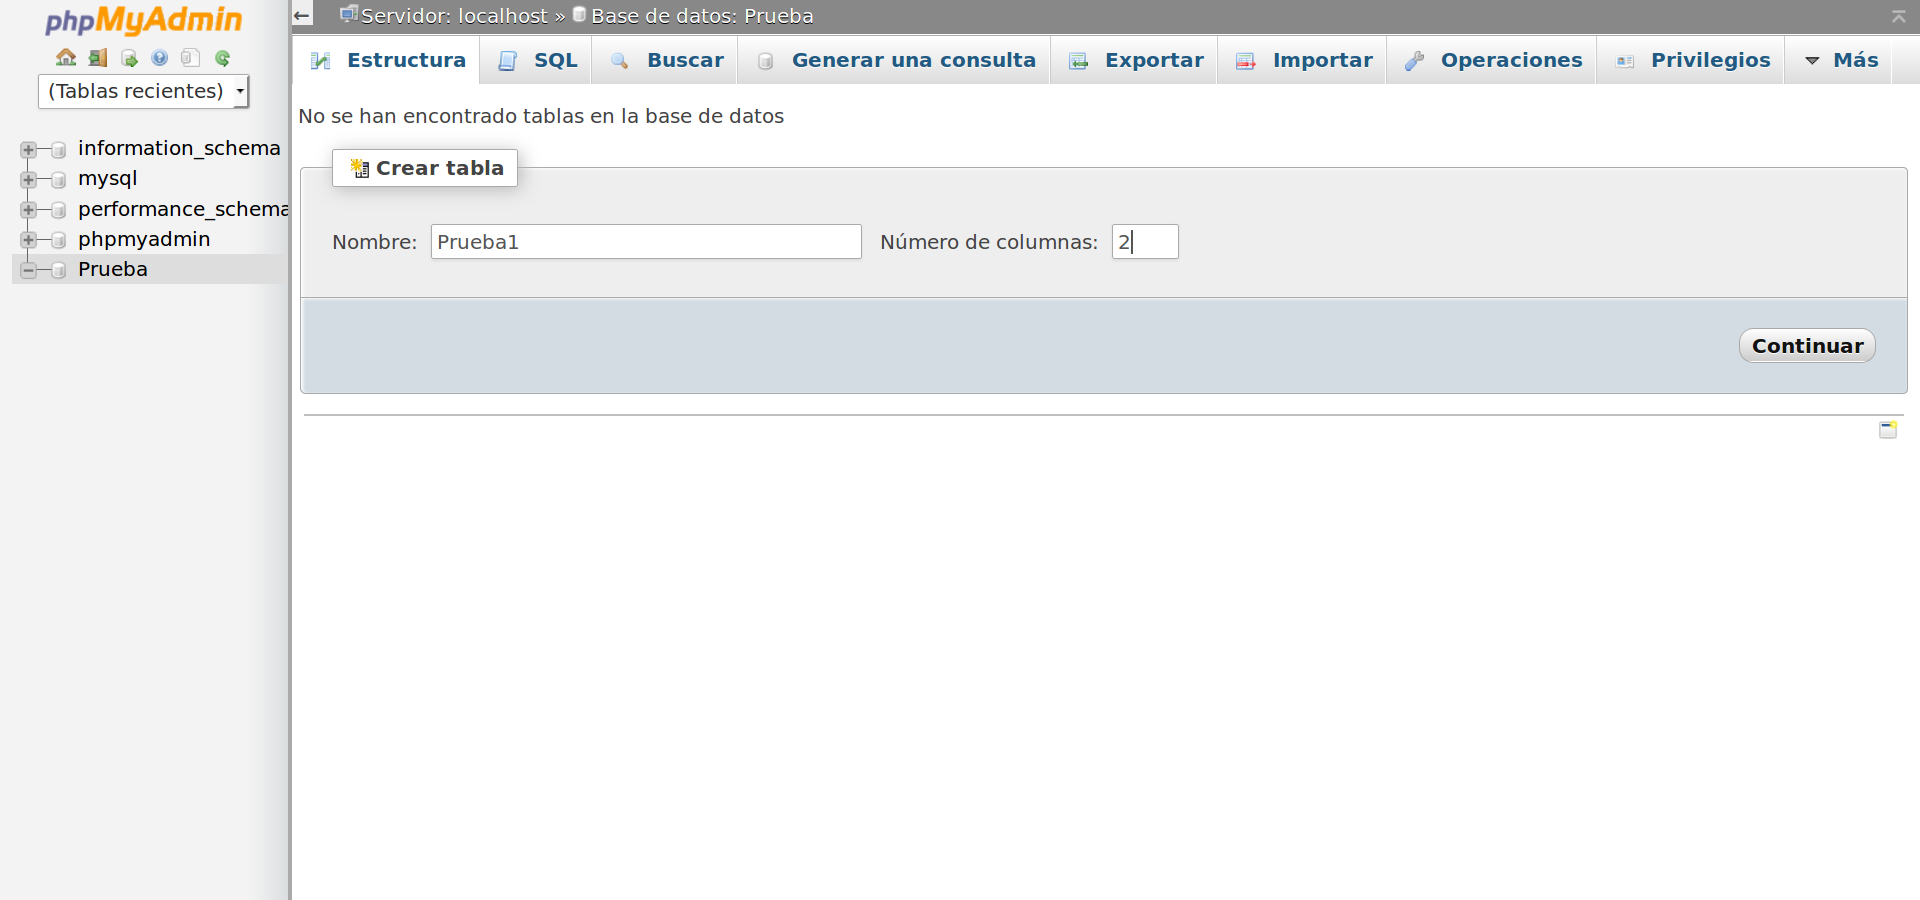
\includegraphics[scale=0.26]{figuras/figura27.png}  %el parámetro scale permite agrandar o achicar la imagen. En el nombre de archivo puede especificar directorios
	\label{figura27}
	
	\caption{Creamos una tabla que se llame Prueba1 con 2 columnas} 
\end{figure}

\begin{figure}[H] %con el [H] le obligamos a situar aquí la figura
	\centering
	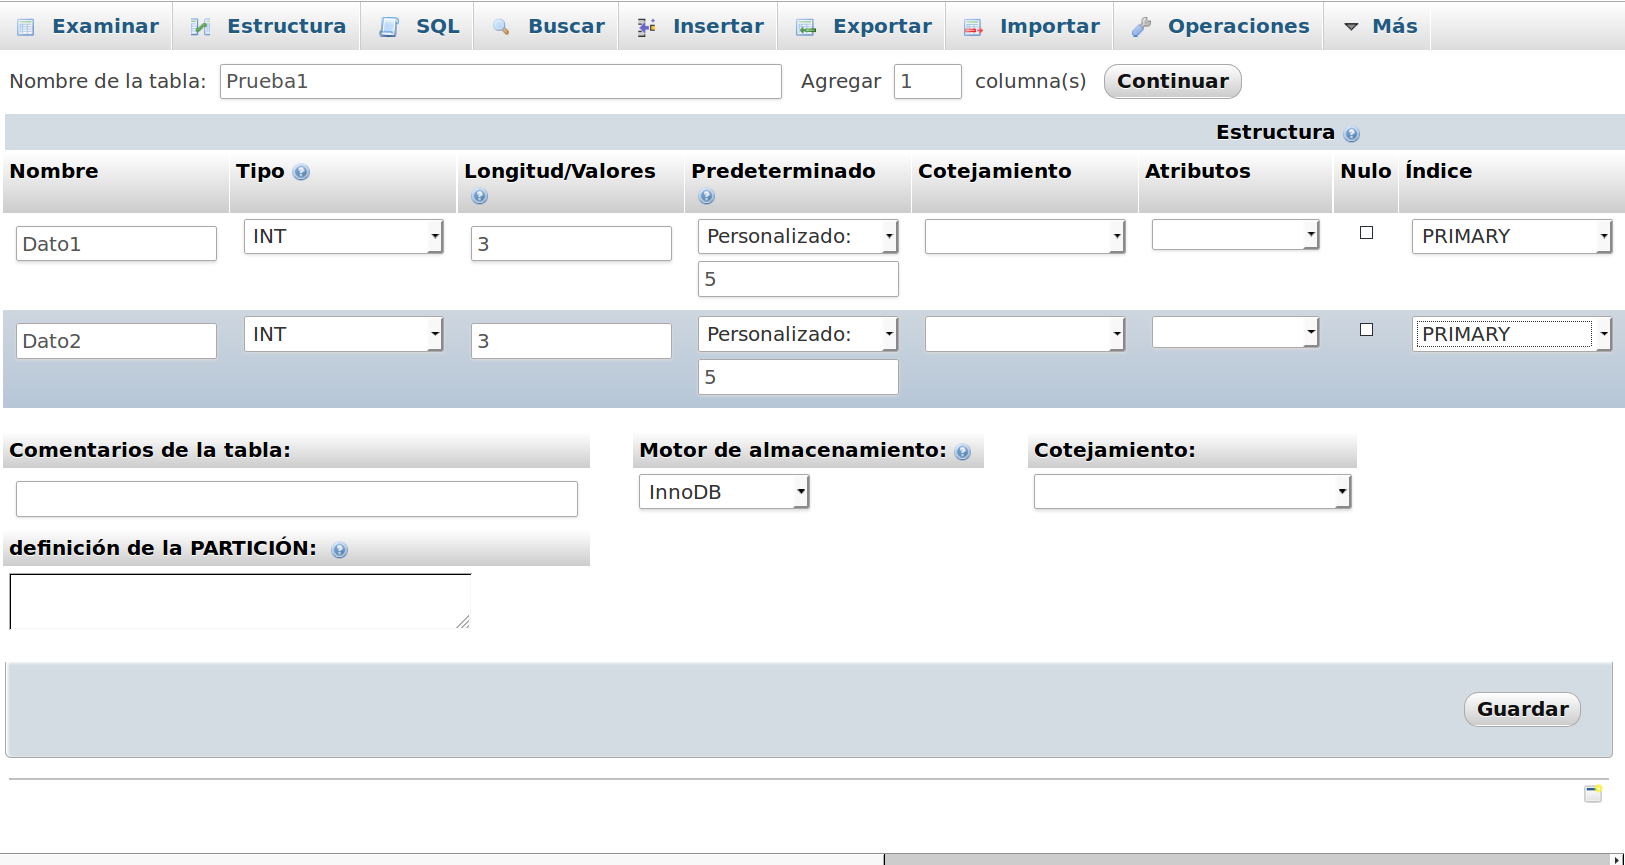
\includegraphics[scale=0.26]{figuras/figura28.png}  %el parámetro scale permite agrandar o achicar la imagen. En el nombre de archivo puede especificar directorios
	\label{figura28}
	
	\caption{Le decimos el valor de los datos de las columnas} 
\end{figure}

La consulta que vamos a realizar de prueba sería:\\

\begin{lstlisting}[language=SQL]

SET profiling=1; --Para decir que vamos a utilizar el profiler
USE Prueba; -- Para indicarle a MySQL la base de datos que vamos a utilizar
select * from Prueba1; -- La consulta, seleccionar todo de la tabla Prueba1
show PROFILES; --Mostramos los datos del profiler

\end{lstlisting}
\begin{figure}[H] %con el [H] le obligamos a situar aquí la figura
	\centering
	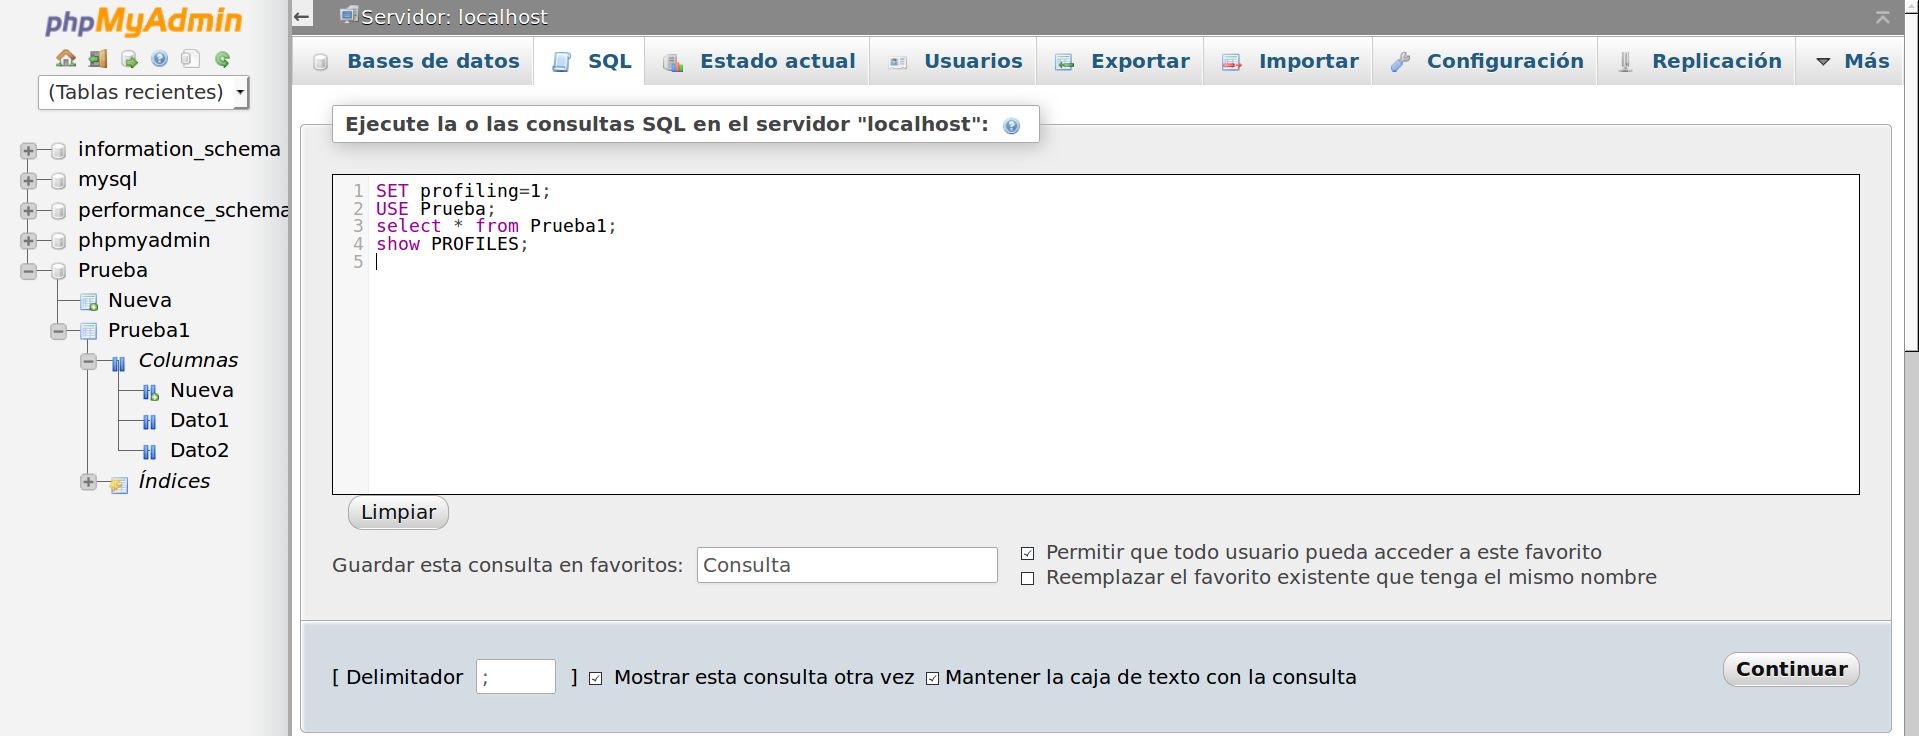
\includegraphics[scale=0.26]{figuras/figura39.png}  %el parámetro scale permite agrandar o achicar la imagen. En el nombre de archivo puede especificar directorios
	\label{figura39}
	
	\caption{Consulta de prueba para el profiler} 
\end{figure}

\begin{figure}[H] %con el [H] le obligamos a situar aquí la figura
	\centering
	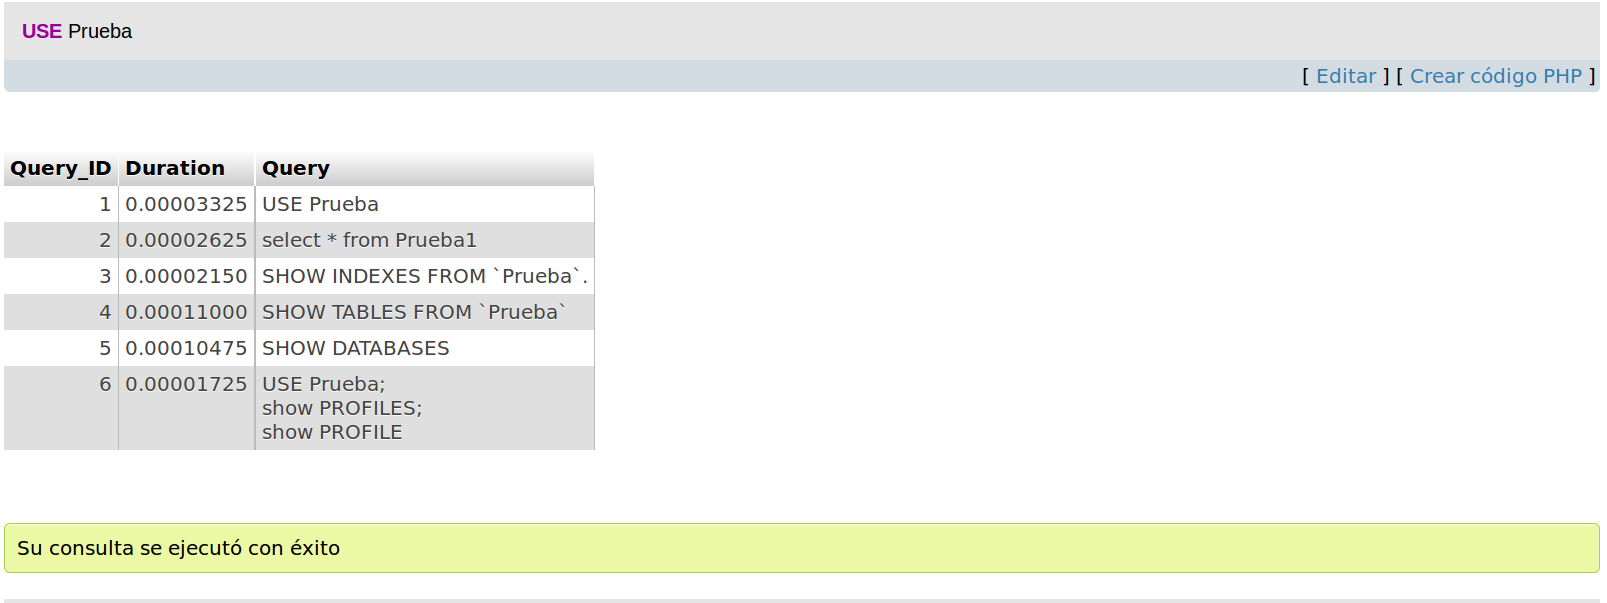
\includegraphics[scale=0.26]{figuras/figura40.png}  %el parámetro scale permite agrandar o achicar la imagen. En el nombre de archivo puede especificar directorios
	\label{figura40}
	
	\caption{Resultado del \textbf{select * from Prueba1;}} 
\end{figure}

En la Figura 9.7 vemos lo que nos devuelve el profiler, que sería:\\
\begin{itemize}
	\item \textbf{starting: } cuánto ha tardado en comenzar.
	\item \textbf{query end: } cuánto ha tardado en terminar.
	\item \textbf{closing tables: } cuánto ha tardado en cerrar las tablas.
	\item \textbf{freeing items: } cuánto ha tardado en liberar los elementos.
	\item \textbf{logging slow query: } cuánto ha tardado en loguearse en la cola lenta.
\end{itemize}
\begin{figure}[H] %con el [H] le obligamos a situar aquí la figura
	\centering
	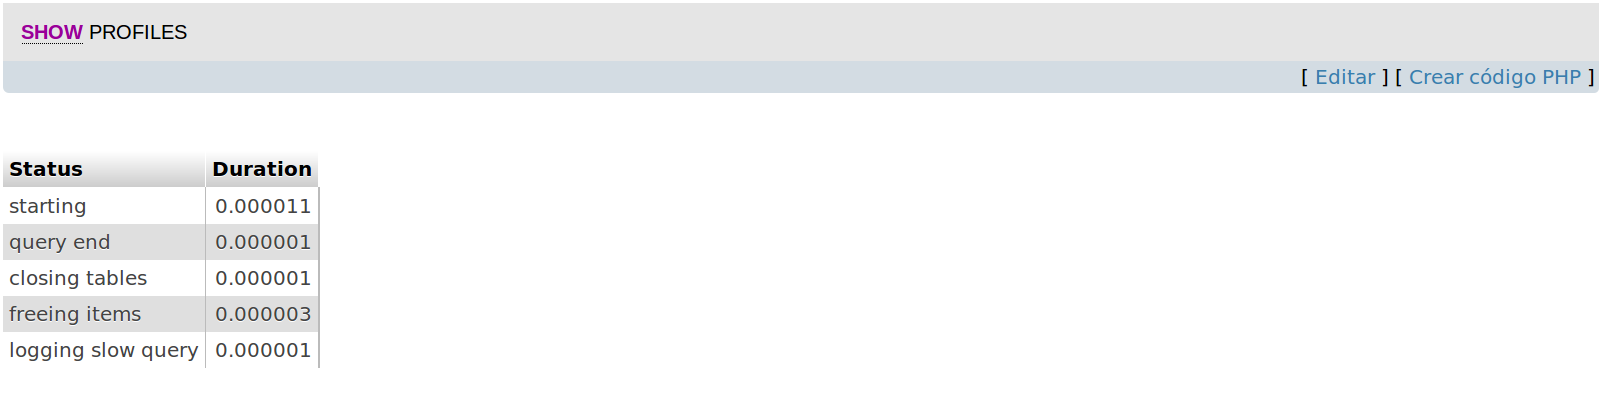
\includegraphics[scale=0.26]{figuras/figura41.png}  %el parámetro scale permite agrandar o achicar la imagen. En el nombre de archivo puede especificar directorios
	\label{figura41}
	
	\caption{Resultado del \textbf{show PROFILES;}} 
\end{figure}

Ahora vamos a probar a hacer la misma consulta, pero en lugar de usar \textbf{show PROFILES;} vamos a utilizar \textbf{show PROFILE ALL;}:\\

\begin{lstlisting}[language=SQL]

SET profiling=1; --Para decir que vamos a utilizar el profiler
USE Prueba; -- Para indicarle a MySQL la base de datos que vamos a utilizar
select * from Prueba1; -- La consulta, seleccionar todo de la tabla Prueba1
show PROFILE ALL; --Mostramos los datos del profiler

\end{lstlisting}

Podemos observar como en la Figura 9.8 obtenemos las mismas filas pero con muchísimas más columnas que nos informan con muchos más datos.

\begin{figure}[H] %con el [H] le obligamos a situar aquí la figura
	\centering
	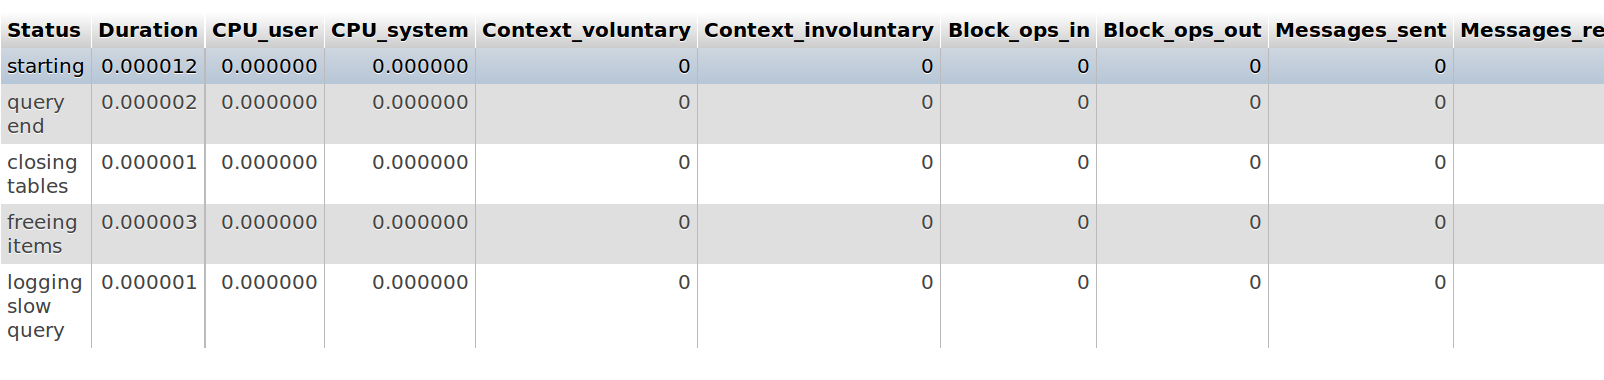
\includegraphics[scale=0.26]{figuras/figura42.png}  %el parámetro scale permite agrandar o achicar la imagen. En el nombre de archivo puede especificar directorios
	\label{figura42}
	
	\caption{Resultado del \textbf{show PROFILE ALL;}} 
\end{figure}
%%%%%%%%%%%%%%%%%%%%%%%%%%%%%%%%%%%%%%%%%%%%%%%%%%%%
% CUESTIÓN OPCIONAL 9
%%%%%%%%%%%%%%%%%%%%%%%%%%%%%%%%%%%%%%%%%%%%%%%%%%%%
\section{Cuestión opcional 9: Escriba un script en python y analice su comportamiento usando el profiler presentado.}
El programa sobre el cuál vamos a ejecutar el profiler es el siguiente:\\

\begin{lstlisting}[language=python]
#!/usr/bin/env python
# -*- coding:utf-8 -*-


repeticiones = 100000

for i in range(repeticiones):
valor = (i * 181728712) / 12787
print("El valor es: ")
print(valor)

\end{lstlisting}

Voy a utilizar el \textbf{CProfile} \cite{pprofiler} para analizar el programa, para ello utilizamos el siguiente comando:\\
\textbf{python -m cProfile  -s 'name'  profiler.py}\\

La opción -s 'name' sirve para ordenarlo por nombre.\\
Y obtenemos el siguiente resultado:\\

\begin{figure}[H] %con el [H] le obligamos a situar aquí la figura
	\centering
	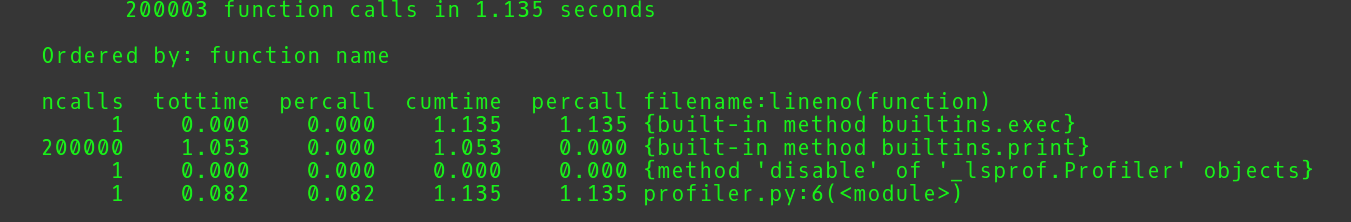
\includegraphics[scale=0.35]{figuras/figura30.png}  %el parámetro scale permite agrandar o achicar la imagen. En el nombre de archivo puede especificar directorios
	\label{figura30}
	
	\caption{Resultados del profiler} 
\end{figure}

Podemos observar que nos encontramos lo primero con el número de llamadas totales y el tiempo de ejecución del programa. En este caso son 200003 llamadas a funciones en 1.135 segundos.\\
Luego nos indica cómo se encuentran ordenada la información que nos muestra, en este caso es por nombre, ya que es como le he indicado anteriormente.\\
Ahora nos encontramos con 6 columnas:
\begin{itemize}
	\item \textbf{ncalls: } número de veces que se llama a la función. En nuestro caso, la primera función que es la \textbf{ejecución} solo se la llama una vez, ya que es la ejecución. La segunda función es \textbf{print} que se le llama 200000, que es el número de veces que itera el bucle for. Y la llamada al \textbf{programa} profiler.py .
	\item \textbf{tottime: } que es el tiempo interno. En este caso sólo tienen valor la llamada a la función \textbf{print} y la llamada al \textbf{programa} .
	\item \textbf{percall: } por llamada. El único campo con valor es el del \textbf{programa}
	\item \textbf{cumtime: } tiempo acumulativo que es el tiempo en total de todas las llamadas de una función. En este caso los valores de la función de \textbf{ejecución} y la de la llamada al \textbf{programa} son los mismos y estos son iguales al valor total del tiempo de funcionamiento del programa. Podemos observar como el otro campo que tiene valor es el de la función \textbf{print}  que vale 1.053, un valor menor al de tiempo total de ejecución.
	\item \textbf{percall: } de nuevo el tiempo por llamada pero esta vez respecto al cumtime.
\end{itemize}

%%%%%%%%%%%%%%%%%%%%%%%%%%%%%%%%%%%%%%%%%%%%%%%%%%%%
% CUESTIÓN OPCIONAL 1
%%%%%%%%%%%%%%%%%%%%%%%%%%%%%%%%%%%%%%%%%%%%%%%%%%%%

\section{Cuestión opcional 1: Indique qué comandos ha utilizado para realizarlo así como capturas de pantalla del proceso de reconstrucción del RAID.}

Para realizar este procedimiento he usado el recurso dado en la pregunta opcional 1 de la práctica 1 \cite{raid}.

\begin{figure}[H] %con el [H] le obligamos a situar aquí la figura
	\centering
	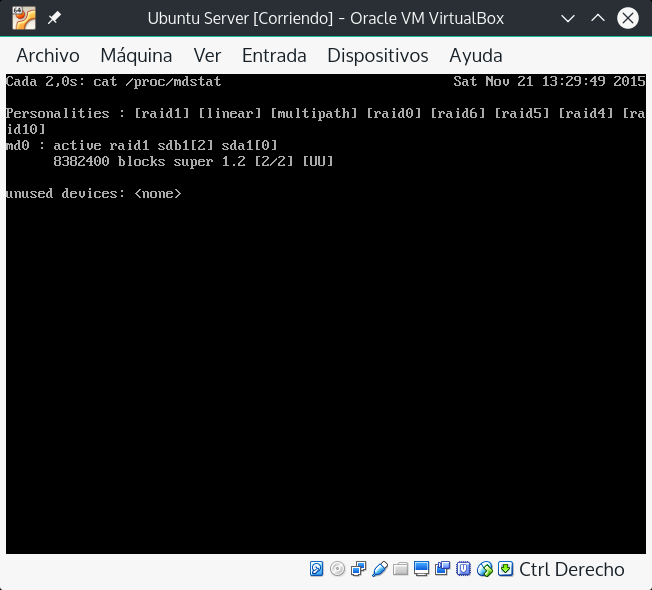
\includegraphics[scale=0.5]{figuras/figura32.png}  %el parámetro scale permite agrandar o achicar la imagen. En el nombre de archivo puede especificar directorios
	\label{figura32}
	
	\caption{Podemos observar cómo tenemos 2 RAID en uso con el comando: \textbf{watch -n2 cat /proc/mdstat}} 
\end{figure}

\begin{figure}[H] %con el [H] le obligamos a situar aquí la figura
	\centering
	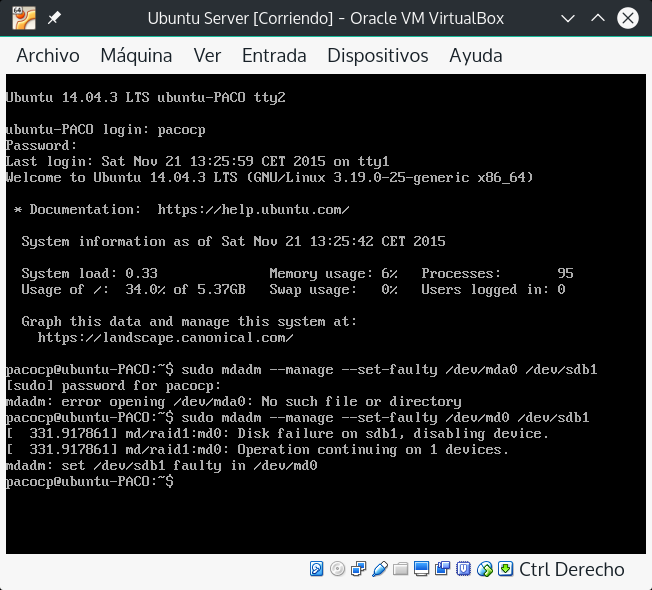
\includegraphics[scale=0.5]{figuras/figura33.png}  %el parámetro scale permite agrandar o achicar la imagen. En el nombre de archivo puede especificar directorios
	\label{figura33}
	
	\caption{Usando el comando \textbf{sudo mdadm --manage --set-faulty /dev/md0 /dev/sdb1} para indicarle que ponga en fallo a sdb1} 
\end{figure}


\begin{figure}[H] %con el [H] le obligamos a situar aquí la figura
	\centering
	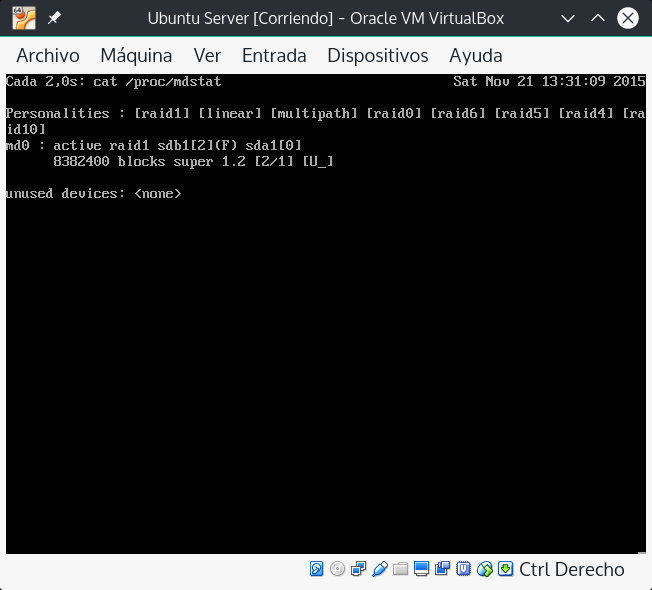
\includegraphics[scale=0.5]{figuras/figura34.png}  %el parámetro scale permite agrandar o achicar la imagen. En el nombre de archivo puede especificar directorios
	\label{figura34}
	
	\caption{Podemos observar cómo ahora en la terminal del watch sólo nos salen 2/1} 
\end{figure}

\begin{figure}[H] %con el [H] le obligamos a situar aquí la figura
	\centering
	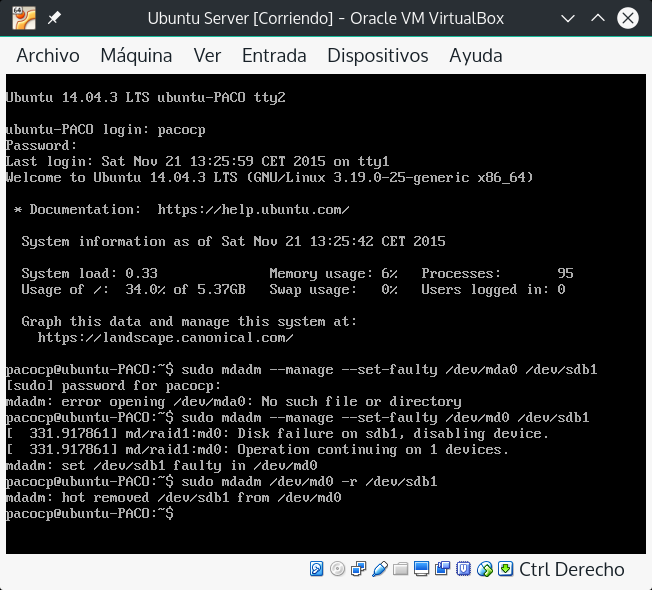
\includegraphics[scale=0.5]{figuras/figura35.png}  %el parámetro scale permite agrandar o achicar la imagen. En el nombre de archivo puede especificar directorios
	\label{figura35}
	
	\caption{Con el comando \textbf{sudo mdadm /dev/md0 -r /dev/sdb1} eliminamos a sdb1} 
\end{figure}

\begin{figure}[H] %con el [H] le obligamos a situar aquí la figura
	\centering
	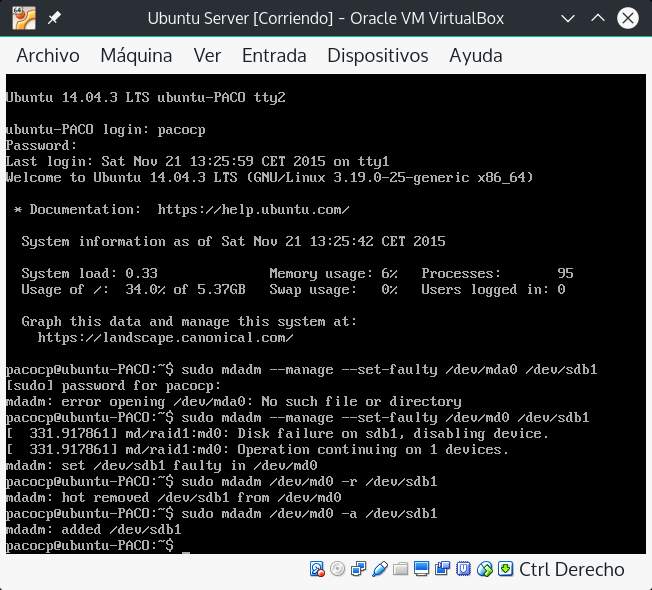
\includegraphics[scale=0.5]{figuras/figura36.png}  %el parámetro scale permite agrandar o achicar la imagen. En el nombre de archivo puede especificar directorios
	\label{figura36}
	
	\caption{Con el comando \textbf{sudo mdadm /dev/md0 -a /dev/sdb1} añadimos de nuevo sdb1} 
\end{figure}

\begin{figure}[H] %con el [H] le obligamos a situar aquí la figura
	\centering
	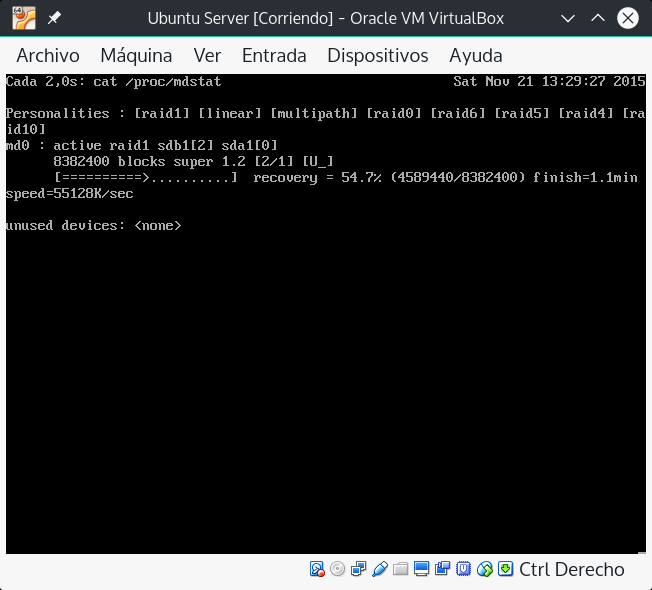
\includegraphics[scale=0.5]{figuras/figura31.png}  %el parámetro scale permite agrandar o achicar la imagen. En el nombre de archivo puede especificar directorios
	\label{figura31}
	
	\caption{Y si nos desplazamos a la terminal com el watch podemos observar como está recuperando el disco} 
\end{figure}

\newpage
\bibliography{citas} %archivo citas.bib que contiene las entradas 
\bibliographystyle{ieeetr} % hay varias formas de citar
\end{document}